%--------------A VOTRE ATTENTION-------------%
% Les étudiants en master qui disposent de plus de 3 chapitres dans leurs travaux peuvent en complèter
% Les Membres doivent figurer dans la dernière version finale du mémoire après soutenance pour dépôt de mémoire

\documentclass{ifri}
\usepackage{titletoc}
\usepackage{ragged2e}
\usepackage{subcaption}
\usepackage[numbers]{natbib}
\justifying
\setlength{\glsdescwidth}{0.65\textwidth}
% \usepackage{lscape}

\typeMemoire{Diplôme de Licence en Informatique}
\optionFormation{Génie Logiciel}
\etudiant{Yélian Joanès Domicov \textbf{AZON}}

\titreDuMemoire{
Conception et implémentation de Numeris229, une architecture logicielle pour un assistant conversationnel intelligent basé sur la génération augmentée par récupération (RAG) : cas du code du numérique en République du Bénin
}

\dateSoutenance{-}
%\promo{2\up{ème}}
\anneeScolaire{2026 - 2027}


%%maitre de mémoire
\encadrants{Armand \textbf{ACCROMBESSI}}

% \jurys{
% \begin{tabular}{llll}
% ~ & ~ & ~ & ~
% \end{tabular}
% }


\hypersetup{
 pdftitle={--},
 pdfauthor={--},
 pdfsubject={--},
 pdfkeywords={--} 
 }

\color{bookColor}

%importation du glossaire
\loadglsentries{glossaire_reduit}

\begin{document}

\pageDeGarde
%\pageTitre

\pagecolor{white}

%% page vide
%\thispagestyle{empty}\ \clearpage


\selectlanguage{french}

% sommaire
\pagenumbering{roman}

\setcounter{tocdepth}{0}
\startlist{toc}
\printlist{toc}{}{\chapter*{Sommaire}}
\setcounter{tocdepth}{5}

%% rdedicaces
% ================= DÉDICACE =================
\cleardoublepage
\thispagestyle{plain}

\vspace*{7cm}

\begin{flushright}
\textit{%
À mes parents,\\
pour leur amour, leur soutien constant\\
et les sacrifices consentis tout au long de mon parcours académique.
}
\end{flushright}
\addcontentsline{toc}{chapter}{Dédicace}
% ===========================================
\newpage 

%% remerciements
\clearpage
\chapter*{Remerciements}
\addcontentsline{toc}{chapter}{Remerciements}
\thispagestyle{plain}

\vspace{1.2cm}

\noindent
Nous tenons à remercier et à témoigner toute notre reconnaissance à
\textbf{DIEU Tout-Puissant}, qui nous a fait Homme et sans qui nous ne
pouvons rien faire. Daigne continuer à poser ton regard miséricordieux
sur nous afin que nous puissions bénéficier davantage de tes grâces.

\vspace{0.4cm}

\noindent
Aussi, nos remerciements iront vers :

\vspace{0.2cm}

\begin{itemize}
    \setlength{\itemsep}{0.35cm}

    \item Prof. Gaston G. EDAH, Directeur de l'Institut de Formation et de Recherche en Informatique (IFRI) ;

    \item Prof. Arnaud AHOUANDJINOU, Directeur-Adjoint de notre institut, pour ses précieux conseils et sa disponibilité à nous accompagner durant la formation ;

    \item Ingénieur Armand ACCROMBESSI, notre maître de mémoire, pour son accompagnement, sa disponibilité, sa confiance et ses précieux conseils tout au long de ce travail ;

    \item Les enseignants de l'Institut de Formation et de Recherche en Informatique, pour la qualité des enseignements dispensés et leur engagement dans notre formation ;

    \item Nos parents, pour leur amour, leurs sacrifices, leur soutien moral et financier ainsi que leur patience ;

    \item Nos frères et sœurs, pour leur affection, leurs encouragements et leur soutien constant ;

    \item Nos camarades de promotion, en particulier ceux qui nous ont apporté leur aide et leurs conseils durant la réalisation de ce mémoire ;

    \item Toutes les personnes qui, de près ou de loin, ont contribué à la réussite de ce travail et dont les noms n'ont pu être mentionnés dans ce document.
\end{itemize}
\newpage 

% Résume
\resume
\selectlanguage{french}
\vspace*{-6cm}
\begin{abstract}
Chaque année, l'accès au code du numérique béninois, texte long et technique régissant les communications électroniques, la protection des données personnelles, le commerce électronique et la cybersécurité, reste difficile pour le citoyen comme pour l'étudiant, faute d'un outil permettant d'y localiser rapidement et fiablement une disposition précise. Cette situation est aggravée par l'existence de lois modificatrices, qui exposent tout lecteur du seul texte d'origine au risque de se fier à un article obsolète. Dans ce contexte, le présent travail propose la conception et l'implémentation de Numeris229, un assistant conversationnel intelligent fondé sur une architecture RAG (Retrieval-Augmented Generation), dont la contribution principale réside dans son ingénierie logicielle. La démarche retenue repose sur un pipeline d'ingestion documentaire reproductible (extraction, contrôle qualité, océrisation, consolidation du texte en vigueur avec ses lois modificatrices, découpage structuré en 629 articles), une indexation vectorielle dans ChromaDB avec le modèle d'embeddings Solon, un module de recherche combinant similarité sémantique et interrogation directe par référence d'article, ainsi qu'une architecture back-end modulaire exposée via une API REST, intégrant la gestion sécurisée des comptes utilisateurs. Le système garantit qu'aucune réponse n'est produite hors du périmètre du corpus indexé, limitant ainsi le risque d'hallucination. Les tests effectués démontrent la capacité du système à restituer des réponses précises et systématiquement sourcées à l'article, tant pour des questions formulées en langage naturel que pour des demandes portant sur un article précis. Cet outil constitue un levier d'accès au droit numérique pour les citoyens béninois, tout en illustrant une démarche de conception logicielle structurée, modulaire et testable pour les systèmes RAG appliqués au droit.

\paragraph{}
\textbf{Mots clés}: RAG (Génération augmentée par récupération), code du numérique, architecture logicielle, droit numérique béninois, assistant conversationnel, ChromaDB.
\end{abstract}

\newpage
\thispagestyle{empty}
\selectlanguage{english}
\addcontentsline{toc}{chapter}{Abstract}
\begin{abstract}

Every year, access to Benin's digital code, a long and technical text governing electronic communications, personal data protection, electronic commerce, and cybersecurity, remains difficult for both citizens and students, due to the lack of a tool enabling quick and reliable retrieval of a specific provision. This situation is compounded by the existence of amending laws, which expose anyone consulting only the original text to the risk of relying on an outdated article. In this context, the present work proposes the design and implementation of Numeris229, an intelligent conversational assistant based on a Retrieval-Augmented Generation (RAG) architecture, whose main contribution lies in its software engineering. The approach adopted relies on a reproducible document ingestion pipeline (extraction, quality control, OCR processing, consolidation of the text in force together with its amending laws, structured segmentation into 629 articles), vector indexing in ChromaDB using the Solon embedding model, a retrieval module combining semantic similarity search with direct querying by article reference, and a modular back-end architecture exposed through a REST API, including secure user account management. The system ensures that no answer is generated outside the scope of the indexed corpus, thereby limiting the risk of hallucination. The tests conducted demonstrate the system's ability to provide accurate, consistently sourced responses at the article level, both for natural language questions and for requests concerning a specific article. This tool constitutes a lever for access to digital law for Beninese citizens, while illustrating a structured, modular, and testable software design approach for RAG systems applied to law.

\paragraph{}
\textbf{Key words}: RAG (Retrieval-Augmented Generation), digital code, software architecture, Beninese digital law, conversational assistant, ChromaDB.
\end{abstract}
\newpage

% ================= LISTE DES FIGURES =================
\cleardoublepage
\listoffigures
\addcontentsline{toc}{chapter}{Liste des figures}


% ================= LISTE DES TABLEAUX =================
\cleardoublepage
\listoftables
\addcontentsline{toc}{chapter}{Liste des tableaux}


% ================= LISTE DES ALGORITHMES =================
\cleardoublepage
\selectlanguage{french}
\listofalgorithmes
\addcontentsline{toc}{chapter}{Liste des algorithmes}


% ================= LISTE DES ACRONYMES =================
\cleardoublepage
\chapter*{Liste des Acronymes}
\addcontentsline{toc}{chapter}{Liste des acronymes}

\begin{center}
\begin{longtable}{p{3cm} p{11cm}}

\textbf{ANSSI} & Agence Nationale de la Sécurité des Systèmes d'Information \\[0.4em]

\textbf{APDP} & Autorité de Protection des Données Personnelles \\[0.4em]

\textbf{API} & Application Programming Interface (Interface de Programmation d'Application) \\[0.4em]

\textbf{CRIET} & Cour de Répression des Infractions Économiques et du Terrorisme \\[0.4em]

\textbf{IA} & Intelligence Artificielle \\[0.4em]

\textbf{JWT} & JSON Web Token (Jeton Web JSON sécurisé) \\[0.4em]

\textbf{LLM} & Large Language Model (Grand Modèle de Langage) \\[0.4em]

\textbf{NLP} & Natural Language Processing (Traitement Automatique du Langage Naturel) \\[0.4em]

\textbf{RAG} & Retrieval-Augmented Generation (Génération Augmentée par Récupération) \\[0.4em]

\textbf{TF-IDF} & Term Frequency - Inverse Document Frequency \\[0.4em]

\textbf{UML} & Unified Modeling Language (Langage de Modélisation Unifié) \\[0.4em]

\end{longtable}
\end{center}

\newpage

% ================= GLOSSAIRE =================
\cleardoublepage
\chapter*{Glossaire}
\addcontentsline{toc}{chapter}{Glossaire}

\begin{description}

\item[Code du Numérique]
Cadre législatif unifié (Loi N° 2017-20 modifiée par la Loi N° 2020-35) régissant l'écosystème numérique, le commerce électronique, les données personnelles, la cybersécurité et les cyberinfractions en République du Bénin.

\item[Cross-Encoder (Reranker)]
Modèle neuronal qui évalue conjointement une question et un extrait de loi pour ré-ordonner les résultats documentaires avec une très grande précision sémantique.

\item[Droit à l'effacement]
Dispositif légal prescrit par le Livre~V du Code du Numérique permettant à tout usager d'exiger la suppression définitive et intégrale de son compte et de ses données personnelles.

\item[Embedding (Plongement vectoriel)]
Représentation mathématique d'un texte sous forme d'un vecteur numérique (768 dimensions pour le modèle Solon), traduisant son sens conceptuel.

\item[Hallucination (IA)]
Fait pour un grand modèle de langage de formuler une réponse factuellement ou juridiquement erronée avec une apparence de certitude.

\item[Large Language Model (LLM)]
Modèle d'intelligence artificielle entraîné sur de vastes corpus textuels pour comprendre et produire du langage naturel (ex.~: \textit{Gemma 3:1b}).

\item[Numeris229]
Plateforme d'information, d'exploration et d'assistance juridique intelligente dédiée au Code du Numérique béninois.

\item[Recherche hybride]
Mécanisme combinant la recherche sémantique dense (par vecteurs) et la recherche lexicale sparse (par mots-clés TF-IDF) pour garantir une extraction documentaire exhaustive.

\item[RAG (Retrieval-Augmented Generation)]
Architecture associant la recherche d'articles de loi officiels à la génération par un modèle de langage pour produire des réponses fiables et sourcées, sans hallucination.

\end{description}


\pagenumbering{arabic}
\setcounter{page}{1}
%%introduction
\chapter*{Introduction Générale}
\addcontentsline{toc}{chapter}{Introduction Générale}

% ── 1. CONTEXTE ET JUSTIFICATION ─────────────────────────────
\section*{ Contexte et justification}
\addcontentsline{toc}{section}{Contexte et justification}

L'accès au droit demeure un enjeu majeur pour l'efficacité des démarches administratives et le renforcement de l'État de droit en République du Bénin. Le code du numérique, institué par la loi n° 2017-20 du 20 avril 2018, modifiée par la loi n° 2020-35 du 06 janvier 2021, régit des domaines aussi variés que les communications électroniques, la protection des données à caractère personnel, le commerce électronique et la cybercriminalité. Ce texte, long de plus de 600 articles répartis en plusieurs livres, titres et chapitres, reste cependant peu consulté par les citoyens, les étudiants et même certains professionnels, en raison de sa longueur, de sa technicité et de la difficulté à y localiser rapidement une disposition précise.

Parallèlement, les avancées récentes de l'intelligence artificielle, notamment les grands modèles de langage (LLM) couplés à des architectures de génération augmentée par récupération (RAG), offrent la possibilité de concevoir des systèmes capables de répondre à des questions en langage naturel à partir d'un corpus documentaire fiable, en citant systématiquement leurs sources. Ces technologies, déjà explorées pour d'autres contextes administratifs et juridiques, n'ont cependant pas encore été appliquées de façon structurée au code du numérique béninois.

C'est dans cette perspective que s'inscrit le projet Numeris229, qui se distingue par son ancrage en génie logiciel : au-delà de la seule performance du modèle d'intelligence artificielle, l'enjeu central de ce travail est de concevoir une architecture logicielle robuste, modulaire et maintenable, capable d'orchestrer l'ensemble de la chaîne applicative — ingestion documentaire, indexation vectorielle, recherche, génération de réponses, gestion des comptes utilisateurs et exposition via une interface de programmation — tout en garantissant la fiabilité, la traçabilité des sources et la sécurité des données.


% ── 2. PROBLÉMATIQUE ─────────────────────────────────────────
\section*{ Problématique}
\addcontentsline{toc}{section}{Problématique}

L'accès au code du numérique se heurte à plusieurs obstacles pratiques. D'une part, la recherche manuelle d'un article précis dans un document de plusieurs centaines de pages est fastidieuse et chronophage, en particulier lorsque l'utilisateur ne connaît ni le numéro ni la terminologie exacte de l'article recherché. D'autre part, l'existence de lois modificatrices, telle que la loi n° 2020-35 qui amende certains articles du texte initial de 2017-20, complique davantage la tâche : un citoyen consultant uniquement le texte d'origine risque de se fier à une disposition obsolète.

Le défi technique consiste donc à concevoir un système capable d'interpréter des questions formulées en langage naturel, de retrouver avec précision les articles pertinents dans un corpus consolidé et à jour, et de produire une réponse fiable, sourcée et compréhensible, sans jamais produire d'information inventée. Au-delà du seul aspect algorithmique, ce défi est également et surtout un défi d'ingénierie logicielle : il s'agit de structurer un pipeline de traitement documentaire reproductible (extraction, océrisation, consolidation, découpage, indexation), de concevoir une architecture back-end modulaire et sécurisée (gestion des comptes, authentification, historique des échanges), et de garantir la qualité et la testabilité de l'ensemble du système.




% ── 3. OBJECTIF GÉNÉRAL ──────────────────────────────────────
\section*{Objectif général}
\addcontentsline{toc}{section}{Objectif général}

L'objectif général de ce travail est de concevoir et d'implémenter Numeris229, une architecture logicielle pour un assistant conversationnel intelligent basé sur une approche de génération augmentée par récupération (RAG), permettant de répondre de façon fiable et sourcée à des questions portant sur le code du numérique en République du Bénin.


% ── 4. OBJECTIFS SPÉCIFIQUES ─────────────────────────────────
\section*{ Objectifs spécifiques}
\addcontentsline{toc}{section}{ Objectifs spécifiques}

Pour atteindre cet objectif général, les objectifs spécifiques sont les
suivants :

\begin{itemize}

    \item[-] Mettre en place un pipeline d'ingestion documentaire reproductible pour le code du numérique, de l'extraction à la consolidation du texte en vigueur, intégrant ses lois modificatrices et un découpage structuré par article ;

    \item[-] Développer un pipeline RAG combinant indexation vectorielle, recherche sémantique et génération de réponses sourcées, capable de refuser de répondre aux questions hors périmètre du corpus ;

    \item[-] Concevoir une architecture back-end modulaire et sécurisée, exposée via une API REST, intégrant la gestion des comptes utilisateurs et l'historique des échanges ;

    \item[-] Développer une interface utilisateur permettant d'interagir avec l'assistant de façon simple et accessible ;

    \item[-] Évaluer la fiabilité et la pertinence du système par la mise en place de tests automatisés couvrant les principaux scénarios d'utilisation.

\end{itemize}


% ── 5. STRUCTURE DU MÉMOIRE ──────────────────────────────────
\section*{Structure du mémoire}
\addcontentsline{toc}{section}{Structure du mémoire}

Ce mémoire présente la démarche de conception de Numeris229 en trois parties. Le Chapitre 1 analyse l'état de l'art des technologies d'intelligence artificielle conversationnelle et des solutions existantes d'accès au droit, et justifie l'approche technique retenue. Le Chapitre 2 détaille l'architecture logicielle et les choix de conception du système, du pipeline d'ingestion documentaire à la gestion des comptes utilisateurs. Le Chapitre 3 présente l'analyse des résultats obtenus et les limites du système.
%\lhead[]{} \rhead[]{} \chead[]{}
\selectlanguage{french}
\fancyhead[L]{\tiny \leftmark}
\fancyhead[R]{\scriptsize \rightmark}
\fancyfoot[C]{\thepage}

\chapter{Revue de Littérature}\label{chap:1}
 \section*{Introduction}
\addcontentsline{toc}{section}{Introduction}

Pour mener à bien le projet Numeris229, il est essentiel d'explorer les concepts théoriques, les technologies et les solutions existantes dans le domaine de l'assistance conversationnelle appliquée à l'accès au droit. Ce chapitre pose les fondements du projet. Il s'articule en quatre sections : une clarification des concepts clés mobilisés, une présentation des approches techniques existantes pour améliorer les systèmes RAG, un état de l'art contextualisant les initiatives d'IA juridique et administrative en Afrique et au Bénin, et une étude comparative de quelques plateformes représentatives du domaine.

\section{Clarification conceptuelle}

\subsection{Agent conversationnel et chatbot juridique}

Un agent conversationnel, communément appelé chatbot, est un programme informatique capable d'interagir avec un utilisateur humain en langage naturel. On distingue les agents à base de règles, dont les réponses suivent des scénarios prédéfinis, des agents à base d'apprentissage automatique, capables de générer des réponses contextuelles à partir de modèles entraînés. Dans le cadre de Numeris229, l'agent conversationnel appartient à la seconde catégorie, augmenté d'un mécanisme de récupération documentaire garantissant que chaque réponse reste ancrée dans le texte officiel du code du numérique, et non dans la connaissance générale, potentiellement erronée, du modèle de langage.

\begin{figure}[H]
\centering

\begin{subfigure}[t]{0.45\textwidth}
    \centering
    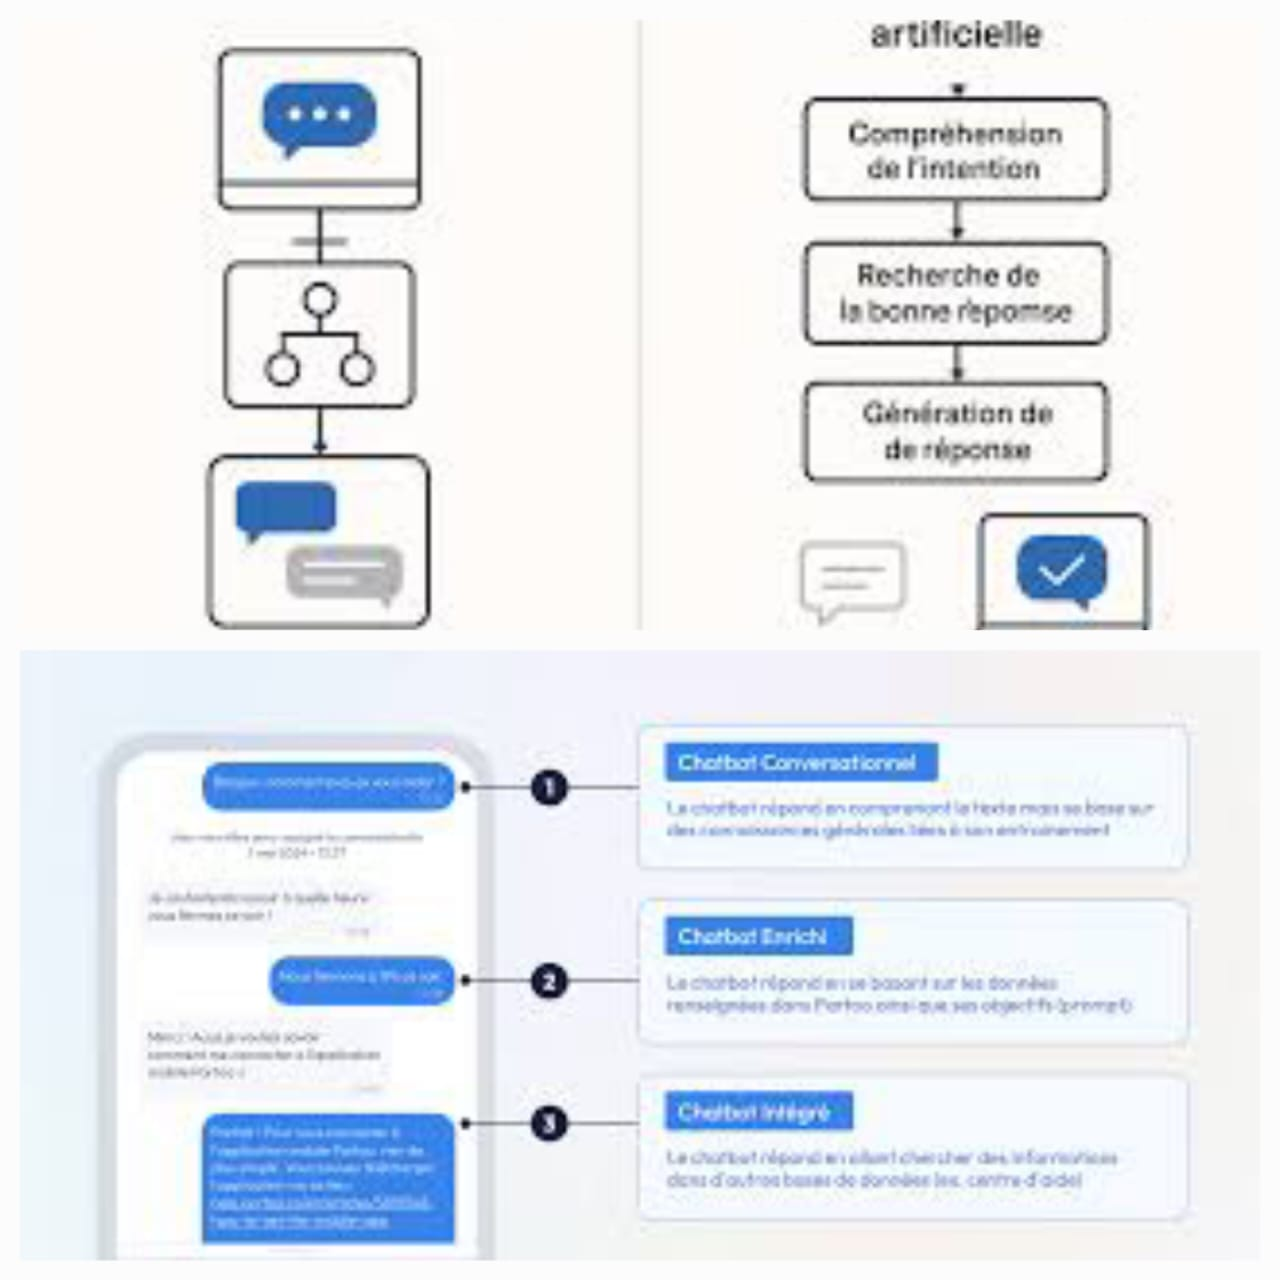
\includegraphics[width=\textwidth]{images/C1/Image2.png}
    \caption{Agent à base de règles}
\end{subfigure}
\hfill
\begin{subfigure}[t]{0.45\textwidth}
    \centering
    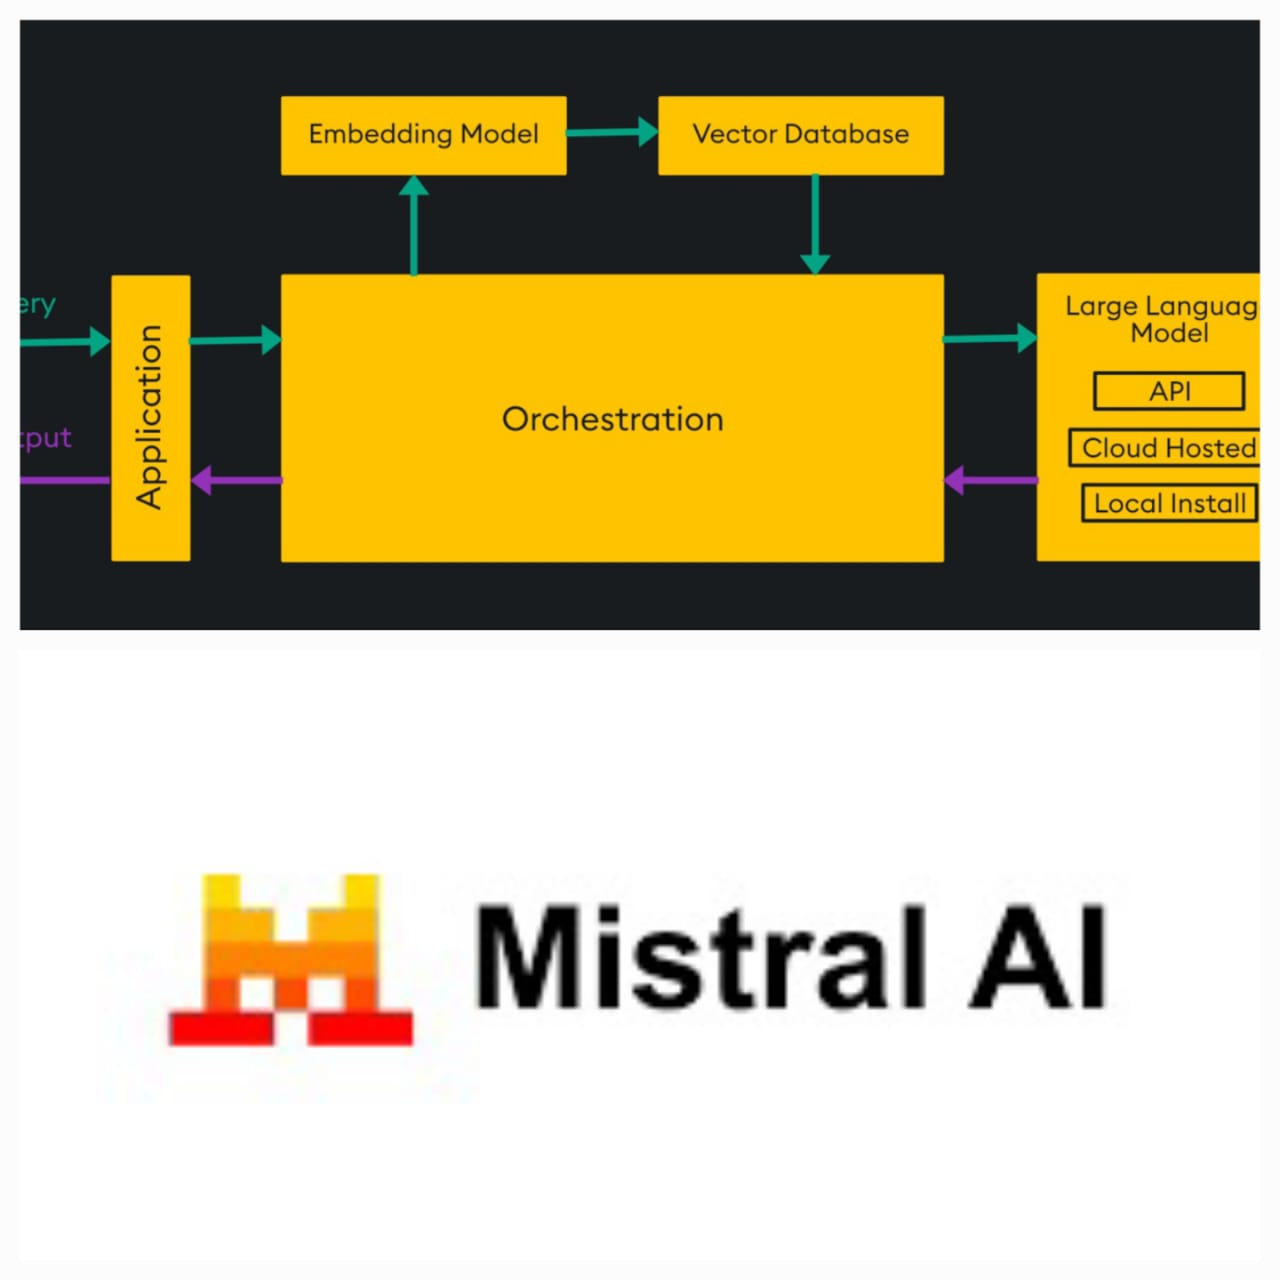
\includegraphics[width=\textwidth]{images/C1/Image1.png}
    \caption{Agent basé sur l’apprentissage automatique}
\end{subfigure}

\caption{Les deux types d’agents conversationnels}
\label{fig:chatbots}
\end{figure}

\subsection{Grands modèles de langage (LLM) et hallucination}

Les grands modèles de langage (LLM) sont des modèles d'apprentissage profond entraînés sur d'importants volumes de texte, capables de comprendre et de générer du langage naturel pour accomplir des tâches variées. Leur principale limite réside dans le phénomène d'hallucination : en l'absence d'ancrage documentaire, un LLM peut produire une affirmation plausible mais factuellement incorrecte. Ce risque est particulièrement critique dans un contexte juridique, où une référence erronée à un article de loi peut induire l'utilisateur en erreur sur ses droits ou ses obligations.

\begin{figure}[H]
\centering
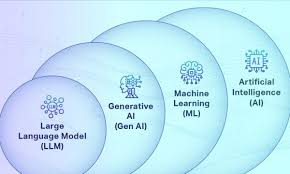
\includegraphics[width=0.6\textwidth]{images/C1/IAG LLM.png}
\caption{IAG et LLM}
\label{fig:chatbot_regle}
\end{figure}

\subsection{Architecture RAG (Retrieval-Augmented Generation)}

L'architecture RAG désigne une approche hybride combinant un module de récupération, qui extrait à partir d'une requête les passages les plus pertinents d'une base documentaire, et un module de génération, qui utilise ces passages comme contexte pour produire une réponse fondée. Pour une question donnée, le système récupère un ensemble de documents maximisant un score de similarité sémantique, puis génère une réponse conditionnée à la fois par la question et par les passages récupérés. Cette architecture garantit que les réponses restent ancrées dans un corpus contrôlé et vérifiable. Dans Numeris229, le corpus est constitué du texte consolidé du code du numérique (loi n° 2017-20 du 20 avril 2018, modifiée par la loi n° 2020-35 du 06 janvier 2021), découpé en 629 articles.

\begin{figure}[H]
\centering
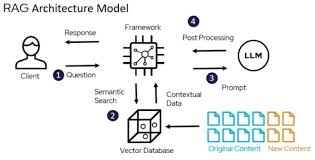
\includegraphics[width=0.6\textwidth]{images/C1/RAG.png}
\caption{RAG}
\label{fig:chatbot_regle}
\end{figure}

\subsection{Embedding et similarité sémantique}

Un embedding est une représentation vectorielle dense d'un texte dans un espace de grande dimension, telle que deux textes sémantiquement proches se trouvent à faible distance l'un de l'autre. La similarité cosinus est la mesure standard utilisée pour comparer ces vecteurs : une valeur proche de 1 indique une forte proximité sémantique. Dans Numeris229, chaque article de loi est transformé en vecteur par le modèle Solon-embeddings-base-0.1, optimisé pour la langue française, et la recherche d'un article pertinent revient à retrouver le vecteur le plus proche de la question posée par l'utilisateur.

\begin{figure}[H]
\centering

\begin{subfigure}[t]{0.45\textwidth}
    \centering
    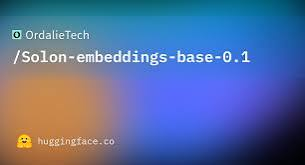
\includegraphics[width=\textwidth]{images/C1/SEB.jpg}
    \caption{Modéle Solon-embeddings-base-0.1}
\end{subfigure}
\hfill
\begin{subfigure}[t]{0.45\textwidth}
    \centering
    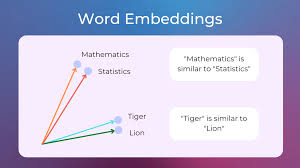
\includegraphics[width=\textwidth]{images/C1/Embedding.png}
    \caption{Embedding avec similarité sémantique}
\end{subfigure}

\caption{Le modèle d'embedding de Mistral et celui avec la similarité sémantique}
\label{fig:chatbots}
\end{figure}

\subsection{Reclassement (reranking)}

Après la phase initiale de récupération, un reranker peut être inséré pour affiner l'ordre des documents selon leur pertinence réelle par rapport à la requête, en s'appuyant sur une architecture de cross-attention qui compare finement la question et chaque passage. Cette étape réduit le bruit transmis au module de génération et améliore la précision des réponses produites.

\begin{figure}[H]
    \centering
    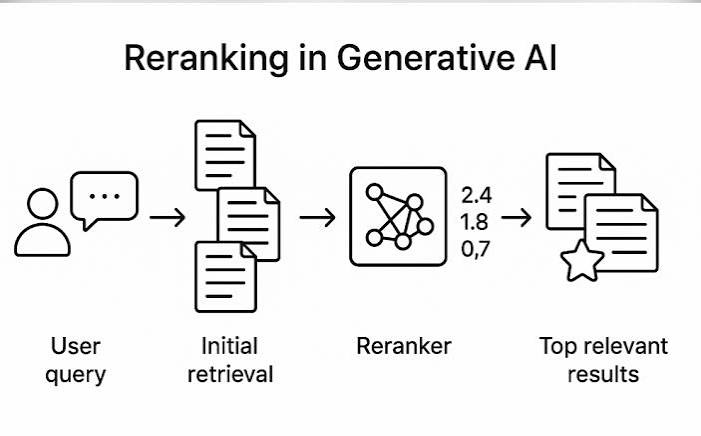
\includegraphics[width=0.45\textwidth]{images/C1/Reranker.jpg}
    \caption{Explication du Reranking}
    \label{fig:reranking}
\end{figure}

\subsection{Droit numérique et cadre juridique béninois}

Le droit numérique désigne l'ensemble des règles encadrant les activités liées aux technologies de l'information et de la communication. En République du Bénin, ce domaine est régi par le code du numérique, qui couvre notamment les réseaux et services de communications électroniques, les services de confiance en l'économie numérique, le commerce électronique, la protection des données à caractère personnel, ainsi que la cybercriminalité et la cybersécurité. Ce texte, structuré en plusieurs livres, titres, chapitres et sections, fait l'objet de modifications ponctuelles par des lois ultérieures, ce qui impose de disposer d'une version consolidée et à jour pour toute exploitation fiable.

\section{Approches techniques d'amélioration des systèmes RAG}

\subsection{Recherche hybride (Hybrid Retrieval)}

La recherche hybride s'impose comme une architecture de référence pour pallier les limites des méthodes de recherche classiques. En combinant la puissance sémantique de la recherche vectorielle avec la précision lexicale de la recherche par mots-clés, elle permet de capturer à la fois le contexte et les termes techniques spécifiques, notamment les numéros d'articles ou les intitulés précis d'une loi.

\subsection{Reclassement des documents récupérés}

Le reclassement des documents extraits par le module de récupération, en fonction d'un score de pertinence plus fin, permet de prioriser les passages réellement utiles avant leur transmission au modèle de génération, réduisant ainsi le risque d'hallucination lié à un contexte bruité.

\subsection{Recherche directe par référence structurée}

Dans un corpus juridique structuré par article, une question mentionnant explicitement un numéro d'article ne bénéficie pas toujours d'une recherche sémantique fiable, le numéro seul portant peu de signal sémantique. Une recherche directe par métadonnée structurée (numéro d'article, livre, titre, chapitre) constitue un complément nécessaire à la recherche vectorielle pour ce type de requête, préoccupation qui rejoint les enjeux d'architecture logicielle centraux à Numeris229.

\subsection{Limites de l'architecture RAG}

L'efficacité d'un système RAG dépend directement de la qualité de la requête utilisateur, de la pertinence des documents récupérés et de la fiabilité de la base de connaissances. Si cette dernière contient des documents obsolètes, non consolidés ou mal structurés, le système peut produire des réponses erronées ou trompeuses, quand bien même l'architecture de génération serait irréprochable. Cette observation justifie l'attention particulière portée, dans Numeris229, à la consolidation du corpus juridique en amont de toute indexation.

\section{État de l'art : IA conversationnelle et accès au droit en Afrique (2018--2026)}

\subsection{Chatbots juridiques généralistes}

Plusieurs chatbots destinés au grand public (Juribot, JuridiqueIA, AideJuridique.ai) proposent une assistance conversationnelle sur des questions de droit, mais restent limités au droit français et ne sont accessibles que par une interface web classique, sans canal de messagerie largement répandu dans les pays à faible connectivité.

\subsection{Plateformes juridiques pour professionnels}

Des plateformes comme Jurisprudence.cc, dédiée à l'espace OHADA, ou LawPavilion/TIMI AI au Nigeria, offrent des capacités avancées d'interrogation de bases juridiques, mais sont destinées aux avocats et magistrats, sur abonnement payant, et ne s'adressent pas au citoyen ordinaire.

\subsection{Chatbots citoyens d'accès à la justice}

Des initiatives comme Wakili.org et LegalBot au Kenya, ou JusticePadi au Nigeria, se rapprochent davantage d'un usage citoyen, intégrant parfois des langues locales. Aucune de ces solutions ne couvre cependant le cadre juridique béninois.

\subsection{Chatbots administratifs gouvernementaux}

Des assistants comme EMY 101 en Côte d'Ivoire ou GovGuideNigeria sont déployés sur des canaux de messagerie largement utilisés, mais se limitent à des démarches administratives sans couverture approfondie d'un texte de loi spécifique.

\subsection{GPT BJ : l'initiative béninoise de référence}

GPT BJ, développée par l'Agence des Systèmes d'Information et du Numérique (ASIN) avec Isheero, constitue la seule initiative d'intelligence artificielle générative souveraine documentée au Bénin. Elle compile notamment les codes des impôts, pénal, du numérique et du travail, et facilite l'accès aux réglementations nationales par le dialogue naturel. Destinée principalement à un usage gouvernemental, elle ne propose pas, à notre connaissance, de canal de messagerie grand public ni de restitution structurée article par article avec traçabilité des sources, fonctionnalités que Numeris229 place au cœur de son architecture.

\subsection{Synthèse et lacunes identifiées}

L'examen de ces initiatives révèle deux lacunes principales pour le cas spécifique du code du numérique béninois : d'une part, l'absence d'un système combinant une couverture exhaustive et à jour de ce texte (incluant ses lois modificatrices) avec une restitution sourcée au niveau de l'article ; d'autre part, l'absence d'une architecture logicielle documentée, modulaire et testable, conçue pour être maintenue et étendue dans la durée plutôt que livrée comme un prototype figé.

\section{Étude de quelques plateformes existantes}

\subsection{GPT BJ (Bénin)}

Développée par l'ASIN, GPT BJ constitue le socle d'IA générative souveraine le plus proche du contexte de Numeris229. Son architecture technique précise n'est pas publiquement documentée, mais sa couverture multi-codes et son absence de canal de messagerie grand public la distinguent d'une solution centrée sur un seul texte, avec une restitution sourcée à l'article.

\subsection{LawPavilion / TIMI AI (Nigeria)}

Cette plateforme offre une recherche avancée de jurisprudence et de textes législatifs ouest-africains, avec une architecture combinant recherche documentaire et génération assistée. Son modèle économique par abonnement et son positionnement à destination des professionnels du droit la rendent peu accessible au citoyen ordinaire, contrairement à l'objectif de Numeris229.

\begin{figure}[H]
\centering

\begin{subfigure}[t]{0.45\textwidth}
    \centering
    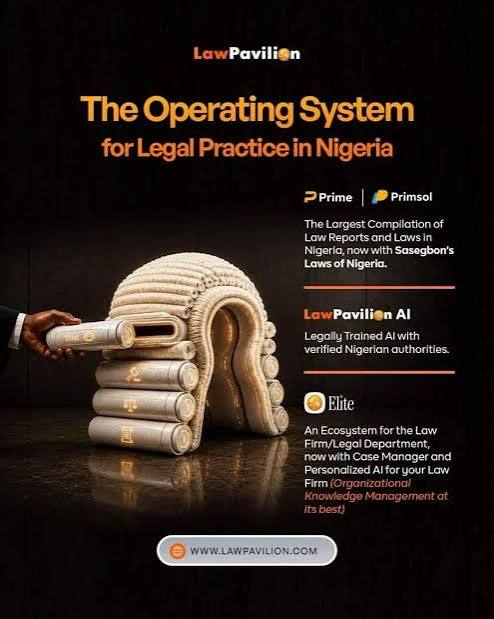
\includegraphics[width=\textwidth]{images/C1/LawPavillon.jpg}
    \caption{LawPavillon}
\end{subfigure}
\hfill
\begin{subfigure}[t]{0.45\textwidth}
    \centering
    
\includegraphics[width=\textwidth]{images/C1/Timi.jpg}
    \caption{Timi AI}
\end{subfigure}

\caption{LawPavillon/Timi AI (Nigéria)}
\label{fig:chatbots}
\end{figure}

\subsection{Wakili.org (Kenya)}

Wakili.org propose une assistance juridique citoyenne via chatbot, avec une attention portée à l'accessibilité linguistique locale. Le système reste cependant circonscrit au cadre juridique kényan et ne constitue pas une solution transposable telle quelle au contexte béninois.

\begin{figure}[H]
    \centering
    
\includegraphics[width=0.45\textwidth]{images/C1/Wakili CRM.jpg}
    \caption{Le chatbot kenyan Wakili.org}
    \label{fig:wakili}
\end{figure}

\subsection{JusticePadi (Nigeria)}

JusticePadi est un assistant conversationnel d'accès à la justice destiné aux citoyens nigérians, disponible sur plusieurs canaux. Son périmètre, centré sur le droit pénal et les droits fondamentaux, ne couvre pas le domaine du numérique.

\begin{figure}[H]
    \centering
    
\includegraphics[width=0.45\textwidth]{images/C1/JusticePadi.png}
    \caption{Le chatbot nigérian JusticePadi}
    \label{fig:justicepadi}
\end{figure}

\subsection{EMY 101 (Côte d'Ivoire)}

EMY 101 est un chatbot administratif gouvernemental déployé sur une messagerie largement utilisée, facilitant l'accès à des démarches administratives courantes. Son architecture illustre la faisabilité technique d'un assistant accessible à grande échelle, mais sans ancrage sur un texte de loi structuré et consolidé.


\begin{figure}[H]
\centering

\begin{subfigure}[t]{0.45\textwidth}
    \centering
    
\includegraphics[width=\textwidth]{images/C1/EMY1.png}
    \caption{EMY1}
\end{subfigure}
\hfill
\begin{subfigure}[t]{0.45\textwidth}
    \centering
    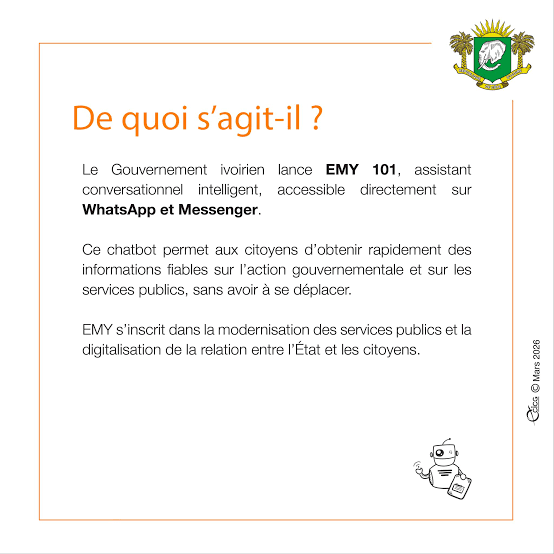
\includegraphics[width=\textwidth]{images/C1/EMY2.png}
    \caption{EMY2}
\end{subfigure}

\caption{Le chatbot EMY 101 de la Côte d'Ivoire}
\label{fig:chatbots}
\end{figure}



\section{Positionnement de Numeris229}

Par rapport aux solutions existantes, Numeris229 se distingue sur plusieurs points. D'abord, par son ancrage documentaire exclusif et consolidé sur le code du numérique béninois, incluant la prise en compte de ses lois modificatrices, ce qui garantit une réponse à jour plutôt qu'une référence à un texte obsolète. Ensuite, par une restitution systématiquement sourcée au niveau de l'article, permettant à l'utilisateur de vérifier l'information à sa source. Enfin, et surtout, par son positionnement affirmé en ingénierie logicielle : au-delà de la seule performance du modèle d'intelligence artificielle, Numeris229 propose une architecture modulaire, sécurisée et testée, de l'ingestion documentaire à la restitution finale, répondant ainsi à la lacune d'architecture logicielle documentée identifiée dans l'écosystème étudié.

\clearpage
\section*{Conclusion}
Ce chapitre a permis de présenter les concepts fondamentaux relatifs à l'intelligence artificielle conversationnelle, à l'architecture RAG et à ses techniques d'amélioration, ainsi qu'au cadre juridique du code du numérique béninois. L'étude des solutions existantes a mis en évidence l'intérêt de ces technologies pour l'accès au droit, tout en révélant l'absence d'une solution combinant couverture consolidée du code du numérique, restitution sourcée à l'article et architecture logicielle robuste et documentée. Cette situation justifie le développement de Numeris229. Les résultats de cette étude constituent une base solide pour la conception de la solution présentée dans le chapitre suivant.

\addcontentsline{toc}{section}{Conclusion}
 
 \chapter{Analyse, Conception et Choix techniques}\label{chap:2}
 \addcontentsline{toc}{section}{Introduction}
\section*{Introduction}

Ce chapitre présente l'analyse des besoins et des contraintes, la conception de la solution ainsi que les choix techniques retenus pour le développement de la plateforme \textit{Numeris229}. Il expose les besoins fonctionnels et non fonctionnels du système, l'architecture générale de la solution, les spécifications conceptuelles au travers des diagrammes UML, ainsi que les choix technologiques justifiés par les impératifs de rigueur juridique, de performance et de souveraineté des données.

% ==========================================================
\section{Analyse des besoins et des contraintes}

\subsection{Besoins fonctionnels}

Les besoins fonctionnels décrivent l'ensemble des services et fonctionnalités que la plateforme \textit{Numeris229} doit fournir afin de faciliter la compréhension, l'accès et l'application du Code du Numérique de la République du Bénin (Loi N° 2017-20 modifiée par la Loi N° 2020-35).

Le système doit permettre :

\begin{itemize}
    \item de collecter, structurer et indexer l'intégralité du corpus juridique officiel du Code du Numérique (Livre Préliminaire et Livres I à VI, soit plus de 600 articles) ;
    
    \item de proposer un explorateur interactif permettant de parcourir, rechercher par mot-clé et filtrer les articles par livre, chapitre ou référence légale ;
    
    \item d'interagir avec les utilisateurs à travers un assistant conversationnel juridique en langage naturel fondé sur une architecture RAG (Retrieval-Augmented Generation) rigoureuse et exempte d'hallucinations ;
    
    \item de détecter automatiquement les questions ciblant un numéro d'article spécifique (ex. « article 55 », « art. 125 ») afin d'assurer une extraction prioritaire et exhaustive du texte légal ;
    
    \item d'effectuer une recherche documentaire hybride combinant recherche sémantique vectorielle (dense) et recherche par mots-clés exacts (sparse TF-IDF) pour garantir une couverture exhaustive des notions juridiques ;
    
    \item de ré-ordonner sémantiquement les articles candidats au moyen d'un modèle de reranking par cross-encoder afin de sélectionner les dispositions légales les plus pertinentes ;
    
    \item de générer des réponses synthétiques, fiables et expressément sourcées, citant obligatoirement le numéro de l'article et le livre concerné ;
    
    \item d'assurer un mécanisme de secours (fallback) restituant fidèlement le texte officiel de loi en cas d'indisponibilité momentanée du service de génération ;
    
    \item d'assurer la gestion complète des conversations (création, historisation, génération automatique du titre, renommage et suppression) dans un espace sécurisé dédié à l'utilisateur ;
    
    \item de gérer l'authentification et le profil des utilisateurs (inscription, connexion sécurisée par jeton, mise à jour des informations personnelles et réinitialisation de mot de passe) ;
    
    \item de garantir l'exercice effectif du droit à l'effacement en permettant la suppression intégrale et définitive du compte utilisateur et de ses historiques.
\end{itemize}

\subsection{Besoins non fonctionnels}

Les besoins non fonctionnels définissent les critères de qualité, de sécurité et d'ergonomie indispensables au bon fonctionnement d'une plateforme d'assistance juridique :

\begin{itemize}
    \item \textbf{Exactitude et fidélité juridique :} élimination stricte des hallucinations grâce à l'ancrage exclusif des réponses dans les textes de loi officiels et à la citation systématique des sources applicables ;
    
    \item \textbf{Sécurité et confidentialité des données :} protection des échanges et des données d'identification conformément aux exigences du Livre V du Code du Numérique et aux recommandations de l'APDP (Autorité de Protection des Données Personnelles du Bénin), avec chiffrement des mots de passe par salage fort (bcrypt) et isolation des sessions ;
    
    \item \textbf{Performance et temps de réponse :} réactivité de l'API REST lors de l'exécution du pipeline RAG grâce à l'indexation matricielle locale des embeddings et au découpage optimisé des contextes ;
    
    \item \textbf{Disponibilité et résilience :} continuité du service assurée par un mode dégradé fluide qui garantit la restitution des articles même lors d'une défaillance du modèle d'inférence ;
    
    \item \textbf{Ergonomie et accessibilité :} interface utilisateur moderne, réactive, dotée d'une prise en charge native des modes clair et sombre, optimisée aussi bien sur ordinateur que sur smartphone ;
    
    \item \textbf{Modularité et maintenabilité :} découpage clair entre les couches de présentation, de traitement d'API et d'intelligence artificielle afin de faciliter l'ajout ultérieur de nouvelles jurisprudences ou décrets d'application.
\end{itemize}

\subsection{Critères d'évaluation}

L'évaluation de l'efficacité et de la précision du système \textit{Numeris229} repose sur les critères suivants :

\begin{itemize}
    \item le taux de précision de l'identification des articles de loi applicables à une requête donnée ;
    
    \item la conformité et la véracité des références légales citées dans les réponses du chatbot ;
    
    \item la réduction effective du taux d'hallucination par rapport à un grand modèle de langage utilisé sans contexte documentaire ;
    
    \item le temps moyen d'exécution du pipeline RAG complet (recherche hybride, reranking et génération) ;
    
    \item la rapidité de chargement et de filtrage au sein de l'explorateur du Code du Numérique ;
    
    \item le taux de réussite des scénarios de test fonctionnels (authentification, gestion des fils de consultation, réinitialisation de mot de passe).
\end{itemize}

\subsection{Contraintes techniques}

Le développement de \textit{Numeris229} est encadré par plusieurs contraintes techniques majeures :

\begin{itemize}
    \item \textbf{Spécificité du vocabulaire juridique béninois :} nécessité d'exploiter un modèle d'embedding adapté à la langue française et au domaine juridique afin de capter la sémantique propre aux textes de loi ;
    
    \item \textbf{Structure hiérarchique complexe de la loi :} découpage rigoureux des 7 Livres en fragments (chunks) préservant le contexte hiérarchique (Livre, Titre, Chapitre, Numéro d'article) sans tronquer les dispositions normatives ;
    
    \item \textbf{Contraintes de souveraineté et d'exécution locale :} déploiement local du modèle d'inférence (LLM) sous Ollama pour préserver la confidentialité des requêtes des usagers et limiter la dépendance envers des API propriétaires tierces ;
    
    \item \textbf{Compatibilité logicielle :} interopérabilité sans couture entre le serveur backend Python (FastAPI) et l'interface utilisateur web développée sous Next.js 14 ;
    
    \item \textbf{Conformité réglementaire :} respect strict des obligations de recueil de consentement et de transparence prescrites par la législation nationale sur la protection des données personnelles.
\end{itemize}

% ==========================================================
% ==========================================================
\section{Conception du système}

\subsection{Démarche de modélisation et architecture générale}

La phase de conception constitue l'étape charnière permettant de traduire l'ensemble des exigences fonctionnelles et des contraintes juridiques en spécifications techniques rigoureuses. Pour mener à bien cette modélisation, le langage standardisé UML (\textit{Unified Modeling Language}) a été retenu et mis en œuvre à travers l'Atelier de Génie Logiciel (AGL) \textbf{Visual Paradigm}. Cet outil professionnel a permis de construire des vues statiques et dynamiques cohérentes, assurant une traçabilité complète entre les besoins des usagers et les composants logiciels implémentés.

L'architecture globale de la plateforme \textit{Numeris229} repose sur un découpage multicouche à couplage faible, garantissant modularité, maintenabilité et haute résilience :
\begin{enumerate}
    \item \textbf{La couche de présentation (Client Web) :} développée sous Next.js 14, elle gère les interactions graphiques, la saisie ergonomique des requêtes, l'affichage réactif des fils de discussion et la gestion du stockage local du jeton d'authentification ;
    
    \item \textbf{La couche applicative et logique métier (Serveur API) :} matérialisée par le framework FastAPI (Python), elle assure le contrôle d'accès, la validation stricte des données entrantes via Pydantic, la gestion des sessions conversationnelles et l'orchestration du moteur RAG ;
    
    \item \textbf{La couche d'intelligence artificielle et d'accès aux données :} elle synchronise une base de données relationnelle SQLite pour les entités transactionnelles et un pipeline RAG composé d'un encodeur sémantique dense (Solon), d'un moteur lexical sparse (TF-IDF), d'un cross-encoder de ré-ordonnancement (CamemBERT) et d'un serveur d'inférence LLM souverain (Ollama).
\end{enumerate}

\subsection{Diagramme des cas d'utilisation}

Le diagramme de cas d'utilisation, élaboré sous Visual Paradigm et illustré à la figure \ref{fig:diagramme_cas_utilisation}, formalise le périmètre fonctionnel du système en adoptant un acteur principal unique : l'\textbf{Utilisateur}. Ce choix de modélisation unifiée traduit fidèlement la réalité de la plateforme : que l'usager soit un citoyen profane désireux de s'informer sur ses droits, un juriste recherchant un article précis, un entrepreneur vérifiant sa conformité e-commerce ou un développeur intégrant des exigences de sécurité, tous partagent les mêmes droits d'accès et exploitent les mêmes fonctionnalités au sein de l'application.

Le système \textit{Numeris229} structure ces fonctionnalités autour de deux grands sous-ensembles :

\subsubsection{Gestion du compte, authentification et conformité}
Ce premier groupe rassemble l'ensemble des cas d'utilisation relatifs à la gestion de l'identité et à la sécurité de l'accès :
\begin{itemize}
    \item \textbf{S'inscrire :} permet à tout nouvel usager de créer un compte sécurisé en renseignant ses données d'état civil et de contact, avec contrôle de complexité et confirmation du mot de passe ;
    
    \item \textbf{Se connecter :} authentifie l'utilisateur via son adresse électronique et son mot de passe, délivrant en cas de succès un jeton d'accès sécurisé JWT (Bearer Token) ;
    
    \item \textbf{Consulter et modifier son profil :} autorise l'usager à vérifier et actualiser ses informations personnelles (âge, profession, numéro de téléphone) ;
    
    \item \textbf{Demander la réinitialisation du mot de passe :} permet en cas d'oubli d'initier une procédure de recouvrement. Ce cas d'utilisation inclut obligatoirement (\textit{<<include>>}) l'action \textbf{Envoyer l'email de réinitialisation}, qui génère un jeton temporaire à durée de validité limitée garantissant la sécurité de la procédure ;
    
    \item \textbf{Réinitialiser le mot de passe :} valide le nouveau mot de passe saisi au moyen du jeton de sécurité préalablement transmis ;
    
    \item \textbf{Supprimer son compte :} fonctionnalité capitale matérialisant le strict respect du droit à l'effacement des données à caractère personnel prescrit par le Livre V du Code du Numérique du Bénin. Cette opération déclenche la suppression intégrale et définitive du compte de l'utilisateur ainsi que de l'ensemble de ses conversations associées.
\end{itemize}

\subsubsection{Consultation juridique intelligente et assistance RAG}
Ce second groupe concentre la valeur ajoutée métier de la plateforme :
\begin{itemize}
    \item \textbf{Créer une conversation :} initialise un nouveau fil de consultation thématique vierge, identifié de façon unique dans le système ;
    
    \item \textbf{Consulter l'historique d'une conversation :} offre à l'utilisateur un accès instantané à la chronologie de ses échanges passés, organisés par date et par titre thématique généré automatiquement ;
    
    \item \textbf{Poser une question :} représente le cas d'utilisation central de consultation en langage naturel. Afin de garantir l'absence totale d'hallucination et l'ancrage juridique strict des explications délivrées, ce cas d'utilisation intègre obligatoirement deux sous-fonctions indispensables via des relations d'inclusion (\textit{<<include>>}) :
    \begin{enumerate}
        \item \textbf{Rechercher les articles pertinents :} étape d'extraction documentaire combinant recherche sémantique dense et recherche lexicale pour isoler les dispositions exactes du Code du Numérique applicables à la question ;
        \item \textbf{Générer une réponse sourcée :} formulation d'une synthèse claire en français formel citant obligatoirement le ou les numéros d'articles et de livres sur lesquels repose l'analyse.
    \end{enumerate}
\end{itemize}

\begin{figure}[H]
  \centering
  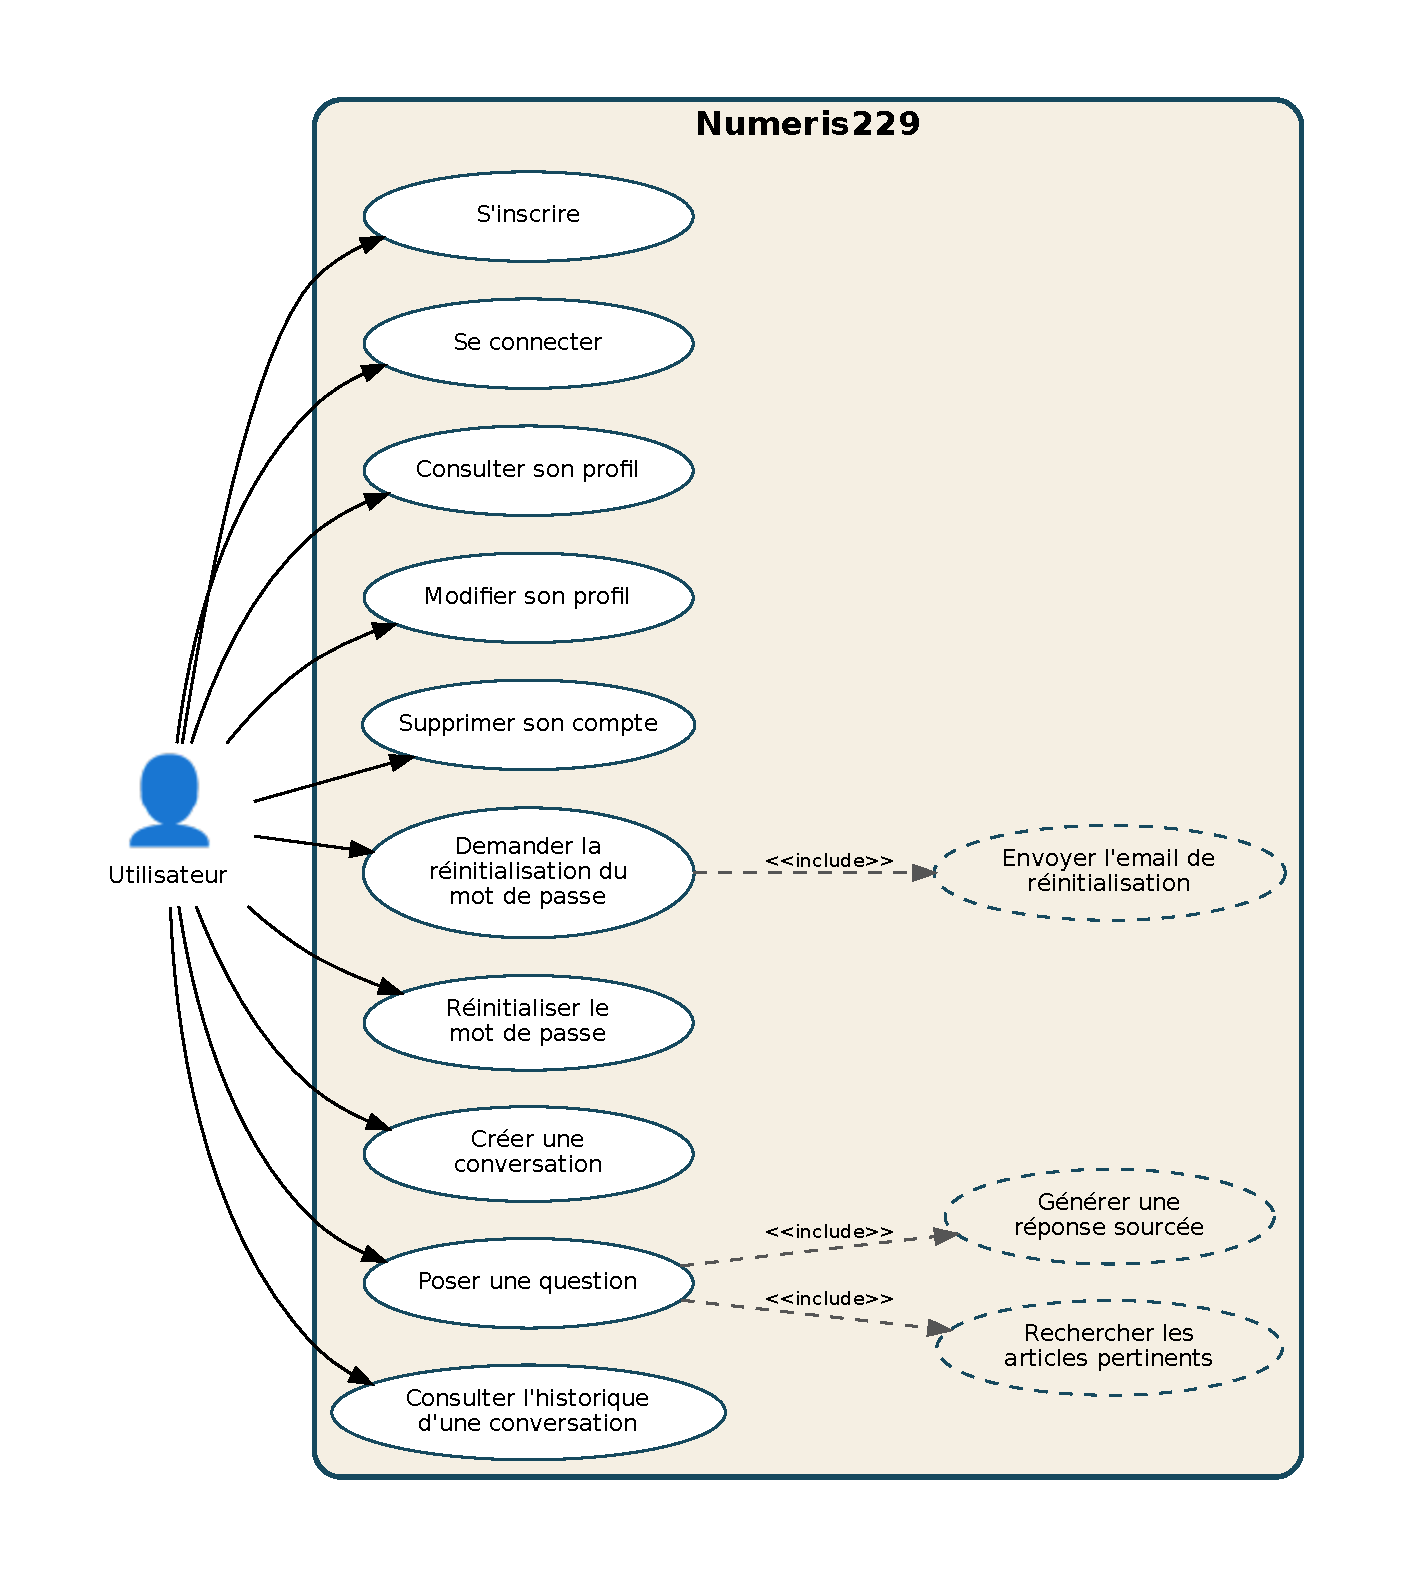
\includegraphics[width=0.85\textwidth]{images/C2/DCU.pdf}
  \caption{Diagramme de cas d'utilisation modélisé sous Visual Paradigm}
  \label{fig:diagramme_cas_utilisation}
\end{figure}

\subsection{Diagramme de classes}

Le diagramme de classes modélisé à la figure \ref{fig:diagramme_classes} expose la structure statique du système, la définition des entités métiers, leurs attributs typés, leurs opérations ainsi que les cardinalités régissant leurs associations.

\subsubsection{Le pôle transactionnel (Espace Utilisateur)}
Ce pôle assure la persistance des interactions au sein de la base de données relationnelle :
\begin{itemize}
    \item \textbf{Classe Utilisateur :} entité maîtresse stockant les informations d'identification (\textit{nom\_prenoms, email, sexe, age, profession, telephone}) et l'empreinte chiffrée (\textit{mot\_de\_passe\_hash}) calculée par hachage salé via l'algorithme bcrypt. Elle encapsule les méthodes de contrôle des identifiants et de purge des données ;
    
    \item \textbf{Classe Conversation :} représente un dossier thématique de consultation. Elle est reliée à la classe \textit{Utilisateur} par une relation de composition forte de multiplicité $1$ vers $0..*$. Cette composition matérialise une dépendance existentielle : une conversation ne peut exister sans son utilisateur propriétaire, et la suppression du compte entraîne automatiquement, par cascade, la suppression de l'ensemble de ses conversations ;
    
    \item \textbf{Classe Message :} constitue l'unité d'échange au sein d'une conversation. Elle conserve la question posée par l'usager, la réponse produite, l'horodatage précis ainsi que la liste des sources juridiques officielles sérialisée au format JSON. Elle est rattachée à la classe \textit{Conversation} par une relation de composition $1$ vers $1..*$.
\end{itemize}

\subsubsection{Le pôle documentaire (Code du Numérique et Chunks RAG)}
Ce pôle modélise la granularité du corpus législatif :
\begin{itemize}
    \item \textbf{Classe Article :} représente chaque disposition unitaire de la Loi N° 2017-20 modifiée. Elle conserve son numéro d'article, son titre, son livre de rattachement, son chapitre ainsi que ses éventuelles mentions de révision législative issues de la Loi N° 2020-35 ;
    
    \item \textbf{Classe ChunkDocumentaire :} matérialise le découpage sémantique d'un article en fragments adaptés aux fenêtres de contexte des modèles d'intelligence artificielle. Chaque chunk est porteur de son texte brut, de son texte enrichi et de ses représentations vectorielles (vecteur dense de dimension 768 et vecteur sparse TF-IDF), permettant le calcul instantané des similarités mathématiques.
\end{itemize}

\begin{figure}[H]
    \centering
    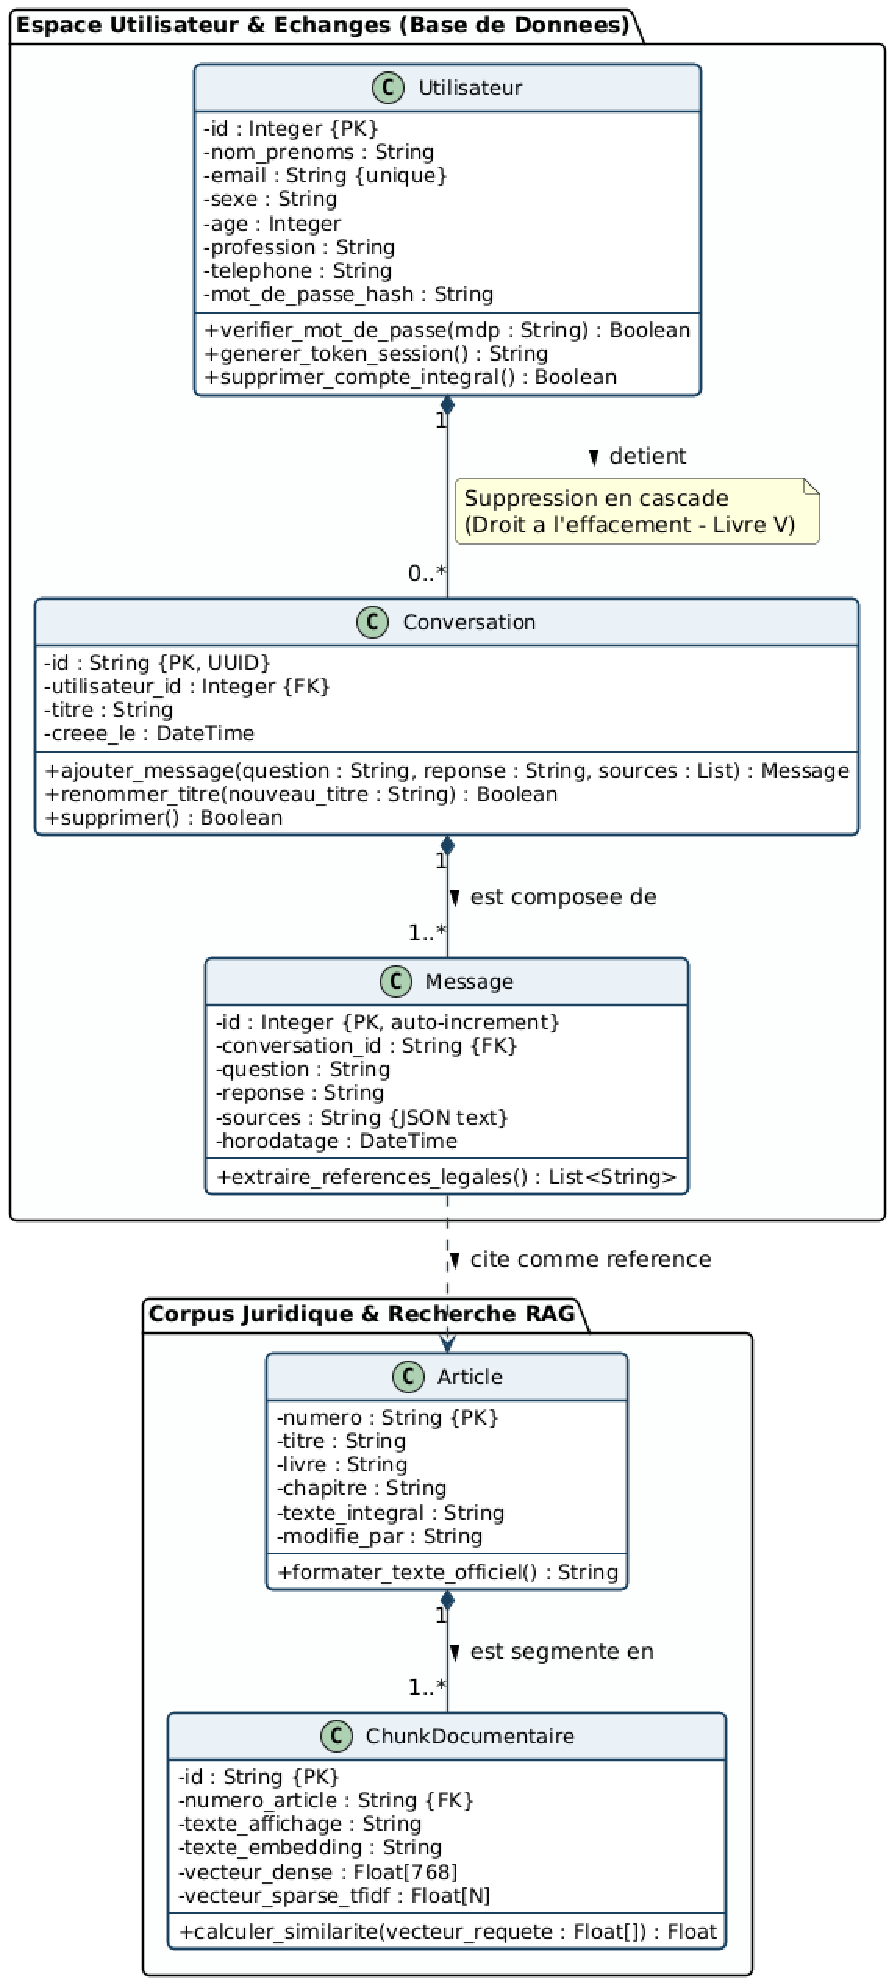
\includegraphics[width=0.95\textwidth]{images/C2/DC.pdf}
    \caption{Diagramme de classes structurel du système Numeris229}
    \label{fig:diagramme_classes}
\end{figure}

\subsection{Diagramme de séquence}

Le diagramme de séquence présenté à la figure \ref{fig:diagramme_sequence} détaille l'enchaînement chronologique des messages et des invocations de méthodes lors du scénario nominal de consultation juridique.

Le cycle de traitement s'articule selon les phases suivantes :
\begin{enumerate}
    \item \textbf{Soumission de la requête :} l'Utilisateur formule sa question en langage naturel sur l'interface Next.js, qui transmet une requête HTTP asynchrone au backend FastAPI en injectant le jeton JWT dans l'en-tête d'autorisation ;
    
    \item \textbf{Vérification d'accès :} le serveur API valide le jeton de session auprès de la base SQLite et transmet la requête à l'orchestrateur \textit{Pipeline RAG} ;
    
    \item \textbf{Routage et recherche documentaire :} l'orchestrateur vérifie si la question contient un numéro formel d'article. En l'absence de numéro explicite, il invoque le \textit{Retriever Hybride} qui calcule simultanément les scores de similarité vectorielle (modèle Solon) et lexicale (modèle TF-IDF) puis extrait les 15 meilleurs chunks candidats ;
    
    \item \textbf{Ré-ordonnancement contextuel :} les 15 candidats sont soumis au modèle \textit{Reranker Cross-Encoder} (CamemBERT) qui opère une évaluation croisée approfondie de chaque extrait vis-à-vis de la question pour ne retenir que les 2 à 3 articles les plus pertinents ;
    
    \item \textbf{Génération souveraine et clause de sauvegarde :} le contexte textuel validé est transmis au serveur local \textit{Ollama} (exécutant le modèle Gemma 3:1B) avec une consigne stricte de citation des articles. Si le serveur d'IA ne répond pas dans le temps imparti (120 secondes), la clause de secours prend immédiatement le relais en extrayant le texte officiel brut sans altération ;
    
    \item \textbf{Persistance et restitution :} le message et ses références légales sont enregistrés en base SQLite, puis retournés au client pour un affichage interactif avec sources dépliables.
\end{enumerate}

\begin{figure}[H]
  \centering
  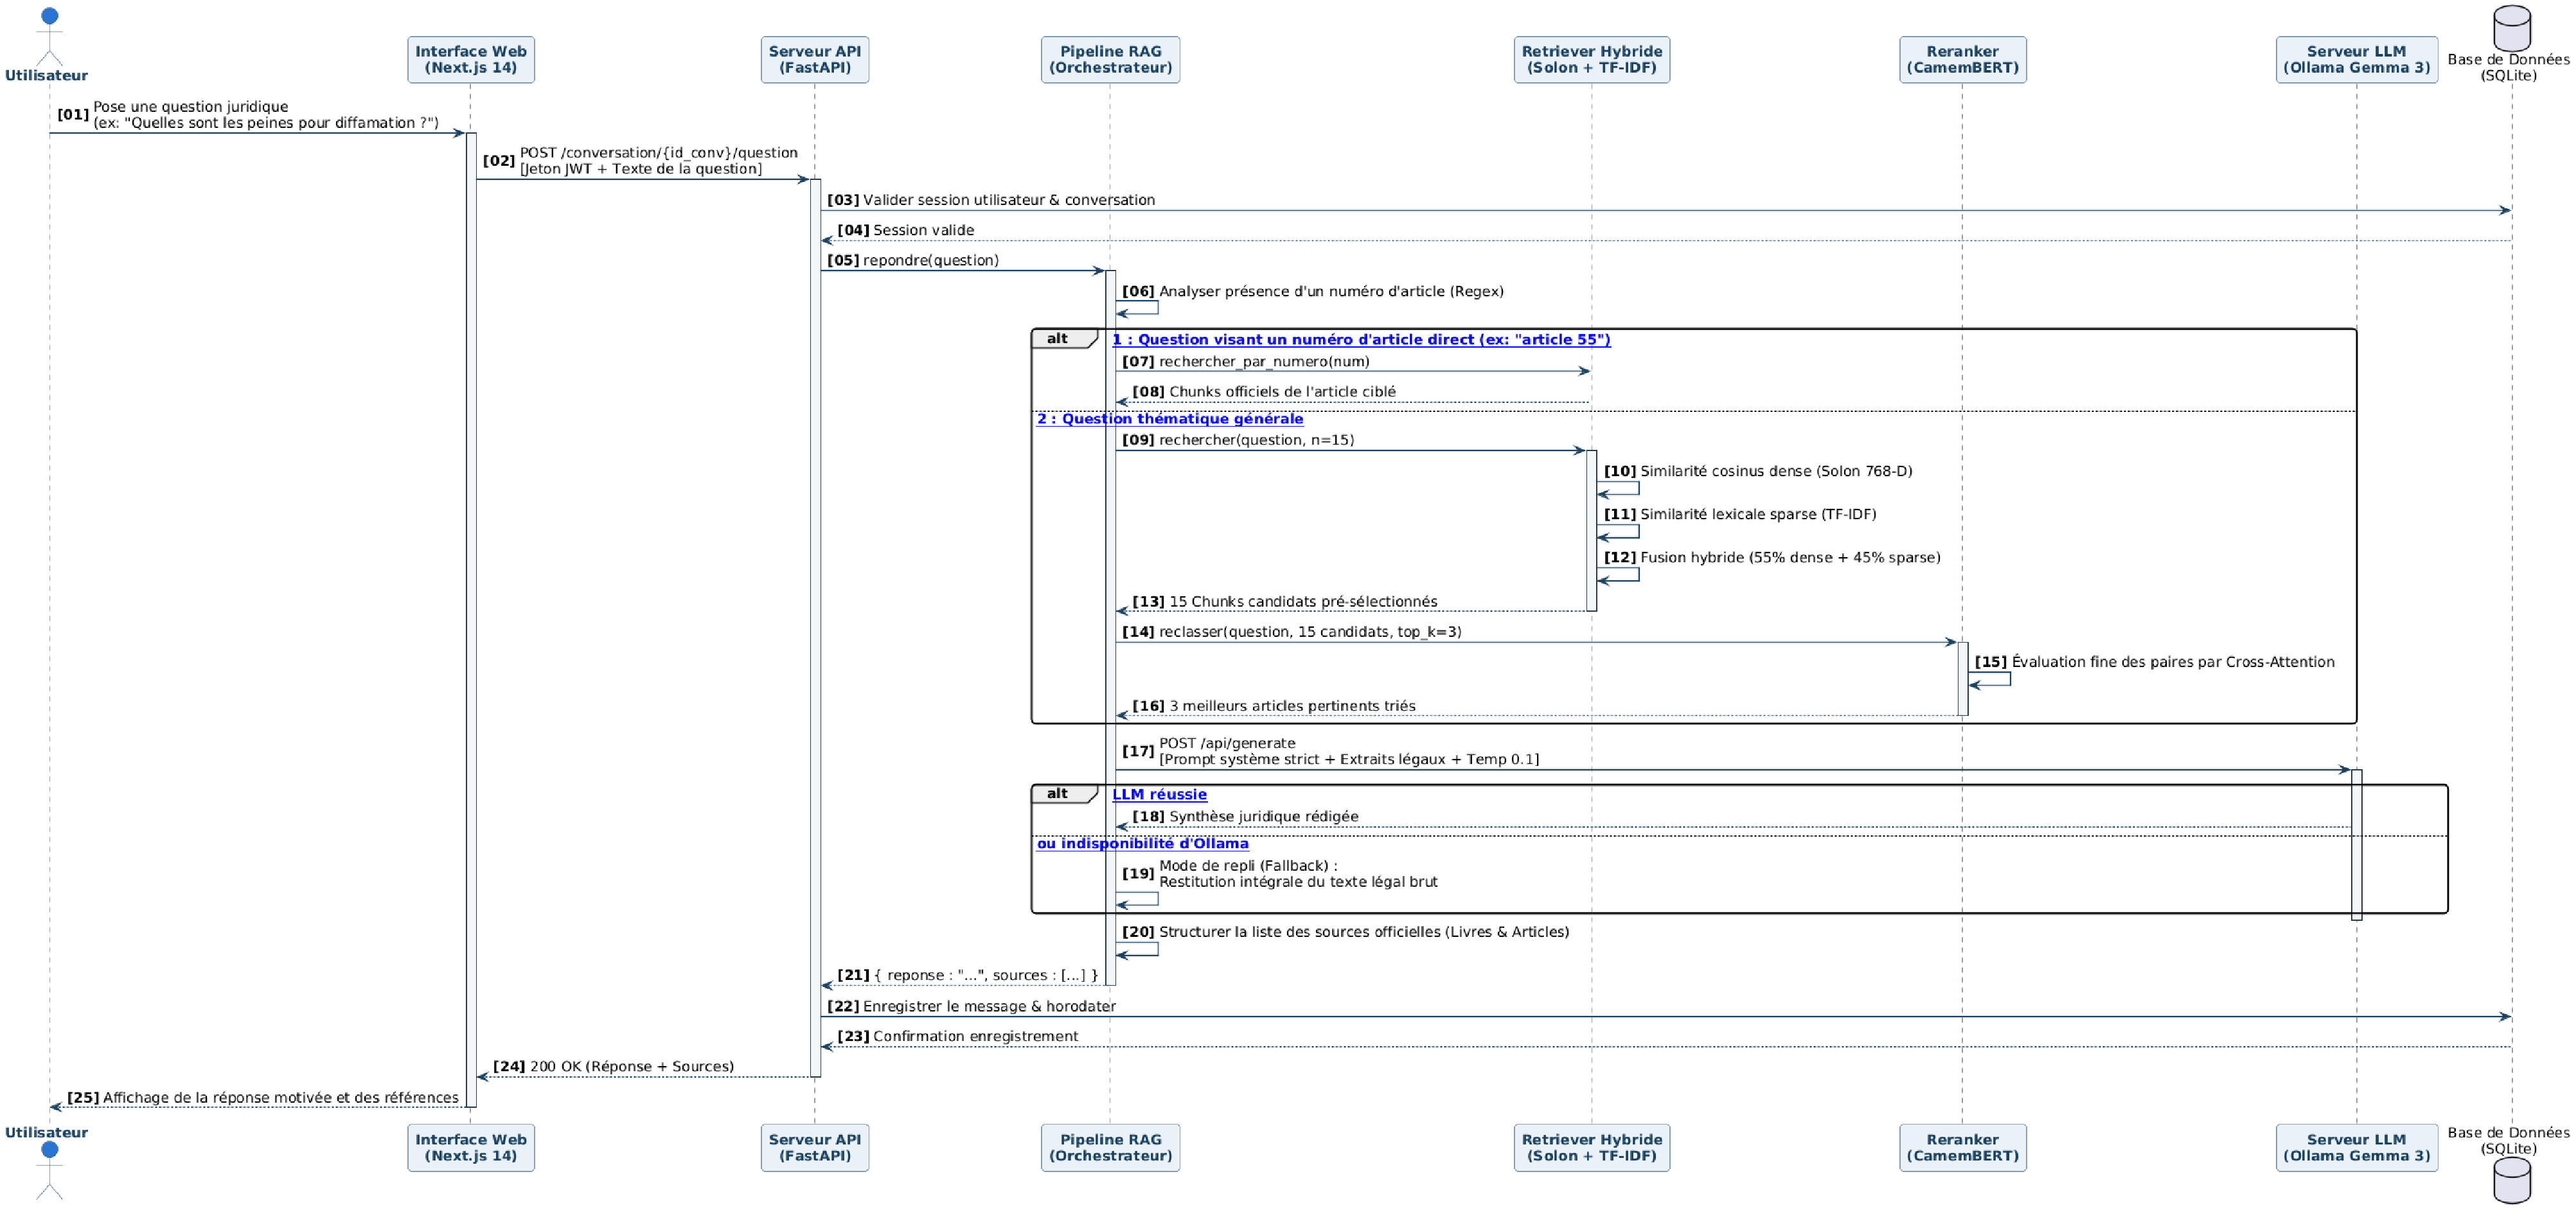
\includegraphics[width=\textwidth]{images/C2/DS.pdf}
  \caption{Diagramme de séquence de la consultation juridique RAG}
  \label{fig:diagramme_sequence}
\end{figure}

\subsection{Diagramme d'activités}

Le diagramme d'activités illustré à la figure \ref{fig:diagramme_activite} cartographie le flux de contrôle opérationnel et les règles de décision conditionnelles appliquées lors de l'exécution d'une requête.

Ce diagramme met en évidence plusieurs mécanismes de sûreté cruciaux :
\begin{itemize}
    \item \textbf{Filtrage d'habilitation initiale :} toute requête émise sans session valide est immédiatement rejetée avec code HTTP 401 et redirection automatique vers l'interface de connexion ;
    
    \item \textbf{Bifurcation selon le type de requête :} le système distingue intelligemment la recherche directe d'article (résolue prioritairement par indexation textuelle exacte) de la recherche thématique sémantique ;
    
    \item \textbf{Parallélisme du Retriever (Fork/Join) :} le calcul dense et le calcul sparse sont exécutés conjointement avant d'être synchronisés pour la normalisation min-max et la fusion pondérée des scores ($55\%$ sémantique / $45\%$ lexical) ;
    
    \item \textbf{Contrôle de pertinence anti-hallucination :} l'algorithme applique une condition de garde stricte sur le score du meilleur candidat ($Score_{max} > -8.0$). Si le sujet n'a aucun fondement dans le Code du Numérique béninois, le système stoppe le pipeline et notifie poliment son incompétence, neutralisant tout risque d'extrapolation trompeuse ;
    
    \item \textbf{Bascule automatique en mode dégradé :} si le modèle de langage subit une défaillance ou un dépassement de délai, le système bascule sans interruption vers la restitution du texte officiel de loi, assurant une disponibilité inaltérable du service.
\end{itemize}

\begin{figure}[H]
    \centering
    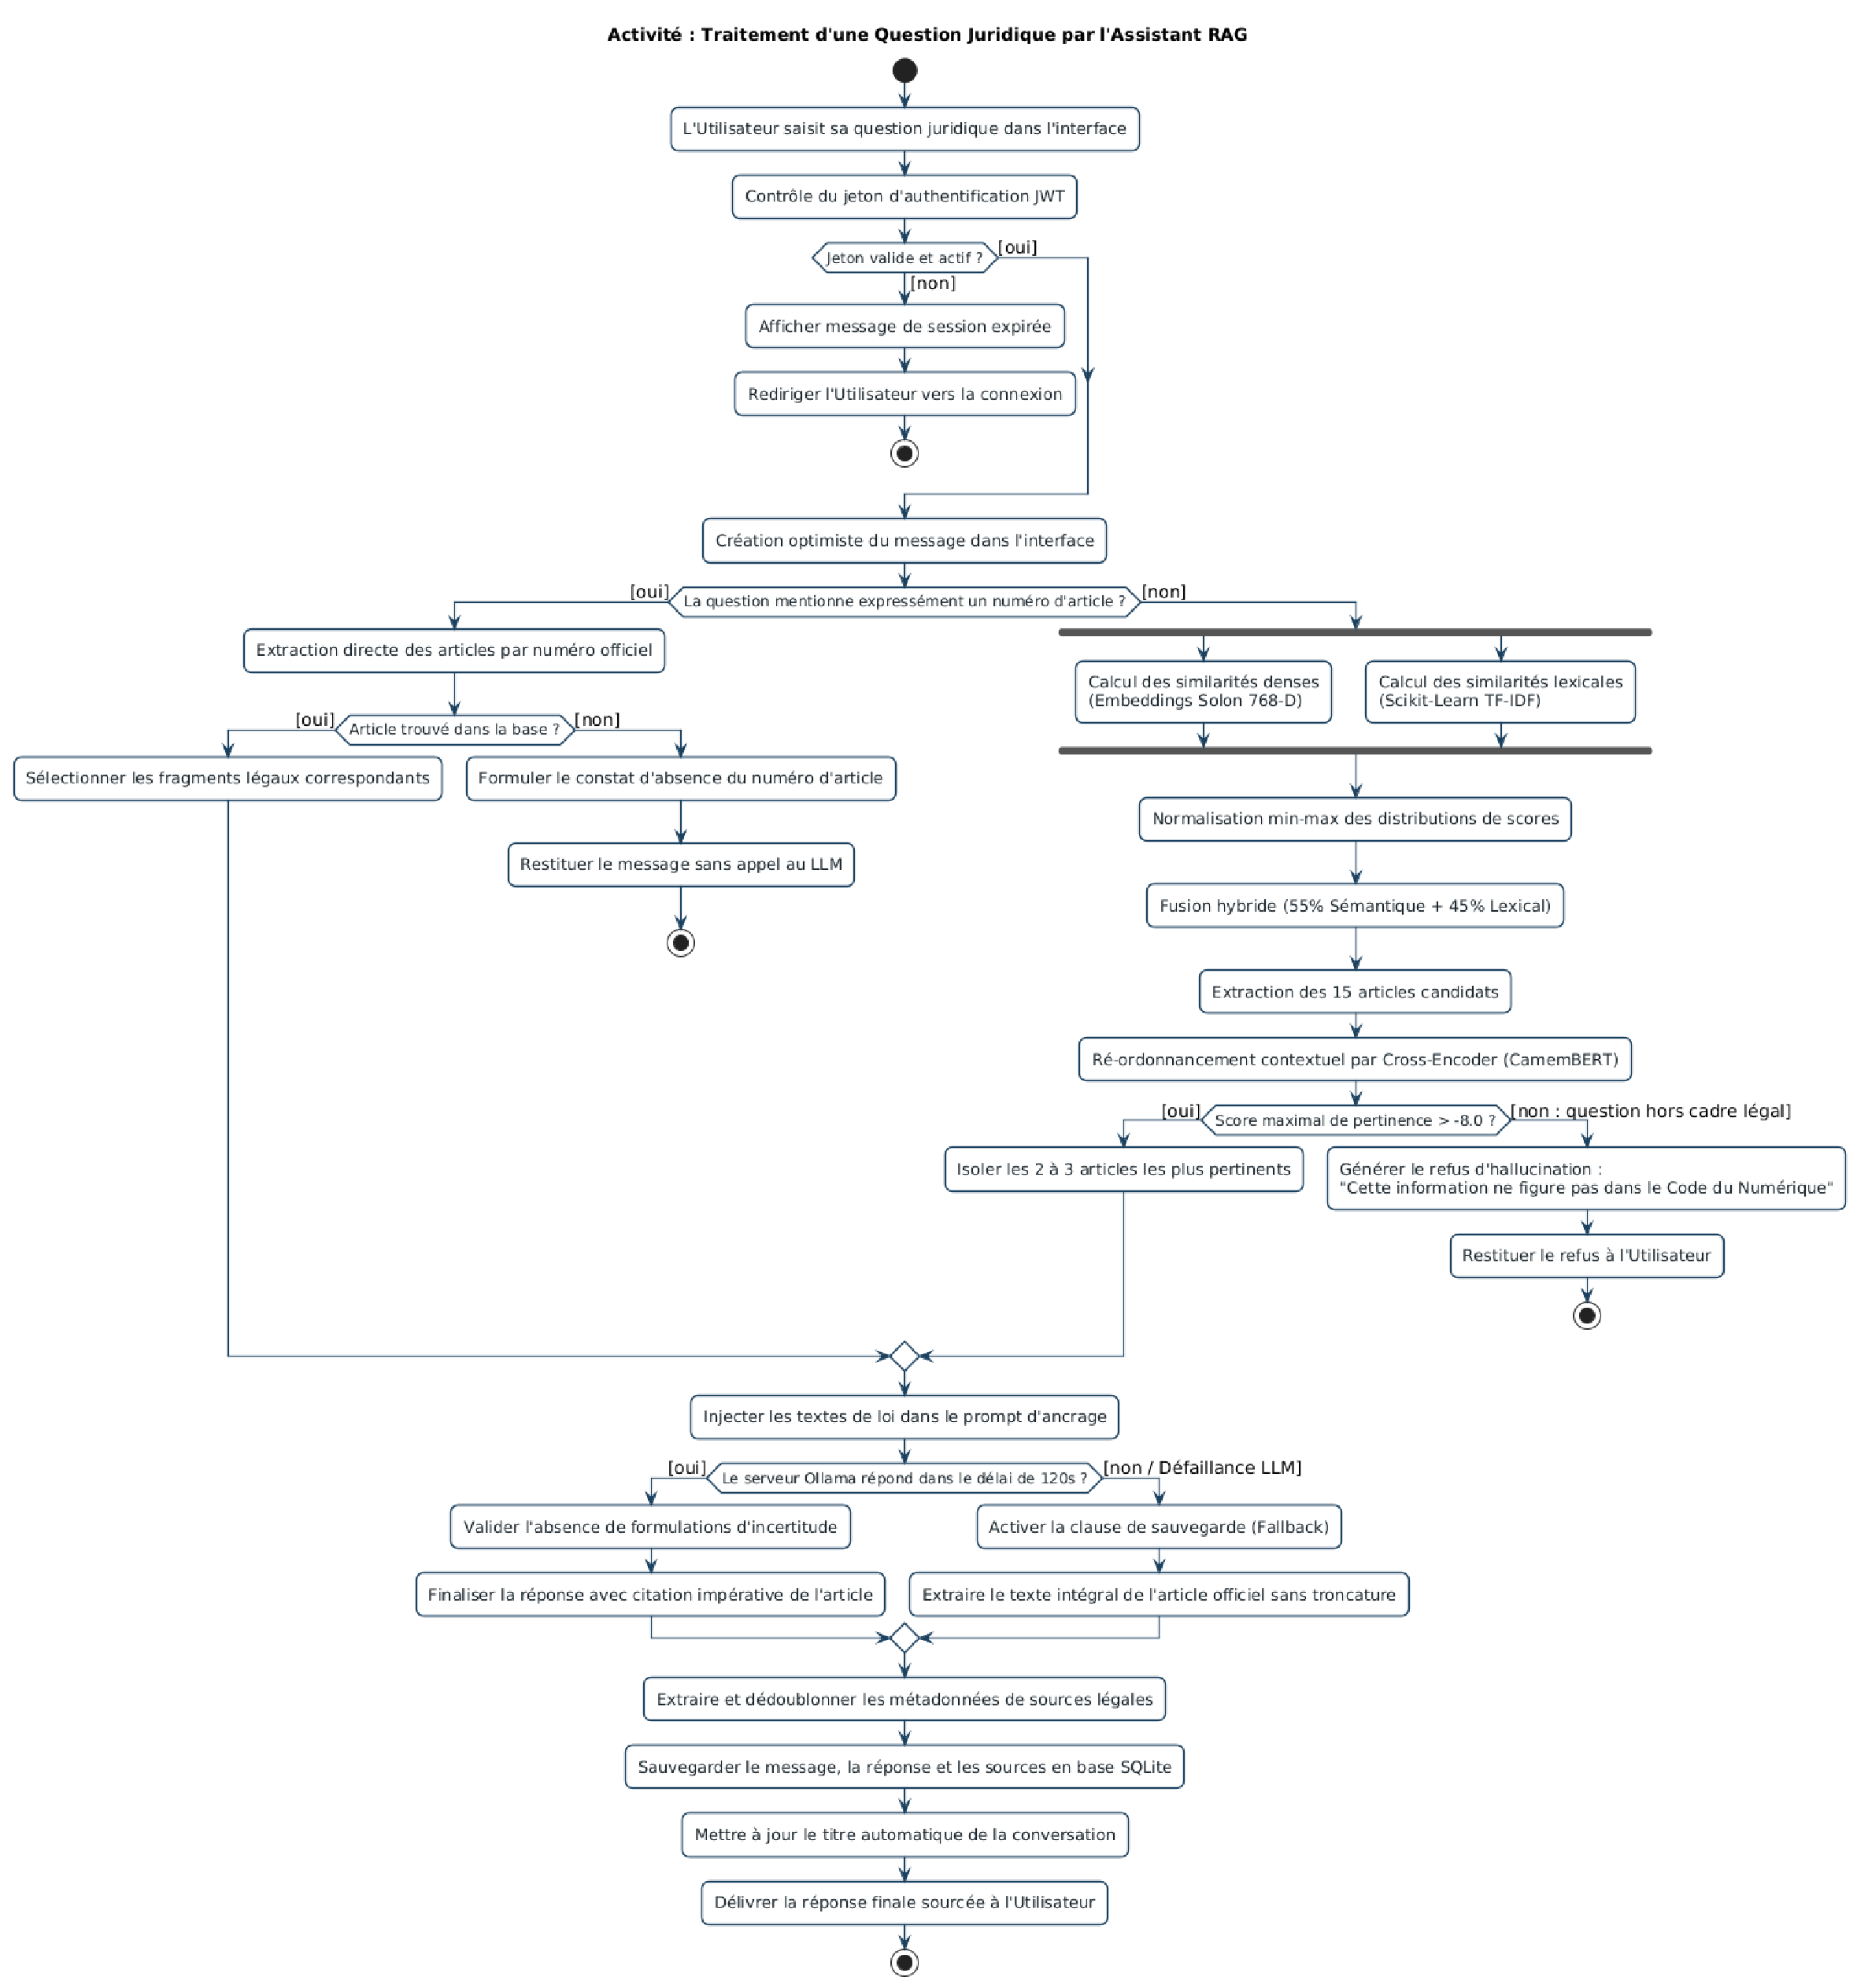
\includegraphics[width=\textwidth]{images/C2/DA.pdf}
    \caption{Diagramme d'activités du processus d'inférence juridique}
    \label{fig:diagramme_activite}
\end{figure}

% ==========================================================
\section{Choix techniques}

\subsection{Justification des technologies utilisées}

Le choix des technologies de \textit{Numeris229} s'appuie sur une analyse multicritères conciliant rigueur scientifique, souveraineté numérique, coût d'infrastructure et conformité aux standards de développement modernes.

\subsubsection{OrdalieTech Solon — modèle d'embeddings juridiques francophones}

La qualité de restitution d'une architecture RAG dépend intimement de la capacité du modèle d'embedding à appréhender les subtilités du vocabulaire juridique. Le modèle retenu est \textbf{OrdalieTech/Solon-embeddings-base-0.1}, un encodeur basé sur SentenceTransformers spécifiquement entraîné sur des corpus juridiques en langue française. Il convertit chaque fragment de texte en un vecteur numérique dense de dimension~768, permettant de capturer les relations sémantiques entre les requêtes profanes et les dispositions normatives du Code du Numérique.

\begin{figure}[H]
    \centering
    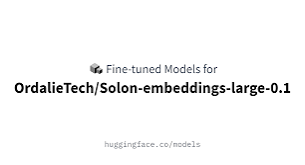
\includegraphics[width=\textwidth]{images/C2/OrdalieTech.png}
    \caption{OrdalieTech Solon}
    \label{fig:ordalietech}
\end{figure}

\subsubsection{Scikit-Learn TF-IDF — recherche lexicale complémentaire}

En matière juridique, la stricte présence d'un terme exact (tel que « diffamation », « signature qualifiée » ou un numéro d'article) est fondamentale. Une recherche purement sémantique peut parfois négliger ces concordances exactes. L'intégration d'un vectoriseur \textbf{TF-IDF} (\textit{Term Frequency - Inverse Document Frequency}) avec analyse des n-grammes $(1, 2)$ permet d'apporter une recherche sparse rapide et précise. La combinaison hybride pondérée ($55\%$ dense Solon et $45\%$ sparse TF-IDF) offre un compromis optimal entre compréhension conceptuelle et exactitude terminologique.

\begin{figure}[H]
    \centering
    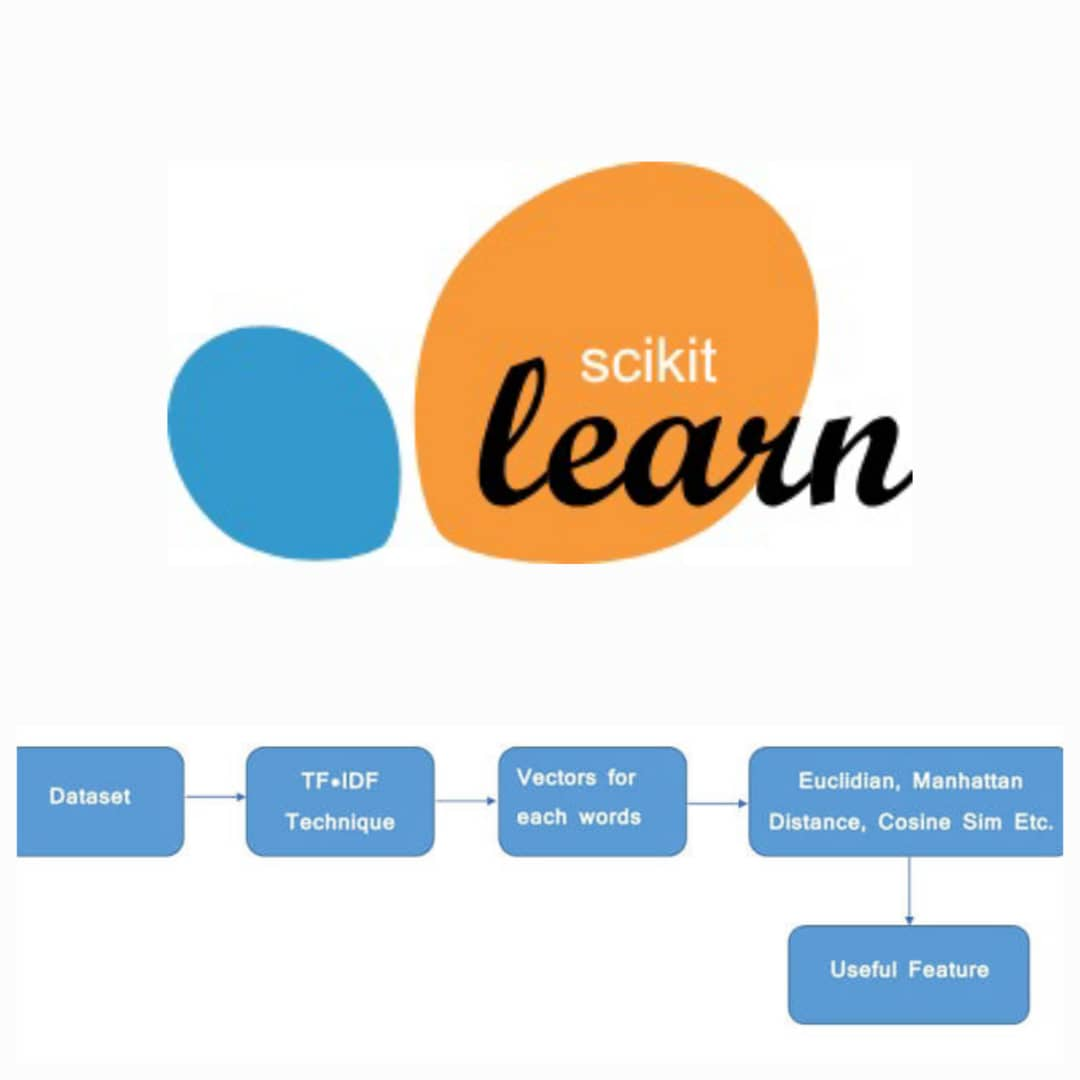
\includegraphics[width=\textwidth]{images/C2/SL-TF IDF.jpeg}
    \caption{Scikit-Learn TF-IDF}
    \label{fig:Scikit-Learn TF-IDF}
\end{figure}

\subsubsection{Cross-Encoder CamemBERT — ré-ordonnancement sémantique (Reranker)}

Pour pallier les limites des modèles bi-encodeurs sur les classements fins, la solution intègre le modèle \textbf{antoinelouis/crossencoder-camembert-base-mmarcoFR}. Contrairement à l'embedding qui traite la question et le document séparément, le cross-encoder évalue la paire question-texte simultanément au moyen de couches d'auto-attention complètes. Il attribue une note de pertinence contextuelle fine à chacun des candidats pré-sélectionnés et permet d'écarter les faux positifs grâce à un seuillage de sécurité strict.

\begin{figure}[H]
    \centering
    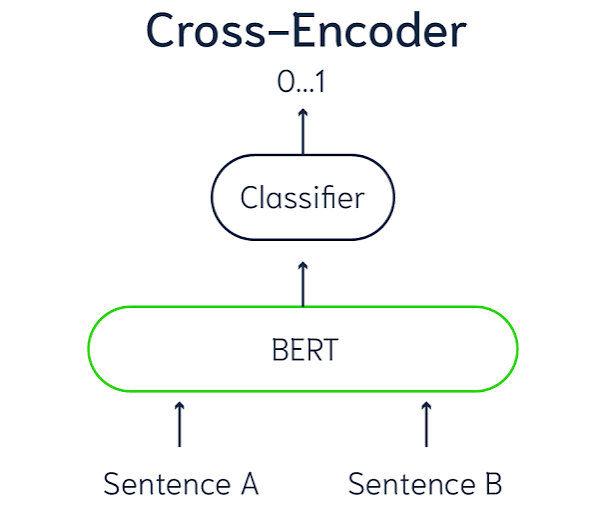
\includegraphics[width=\textwidth]{images/C2/CrossEncoder.png}
    \caption{Schema du reranker}
    \label{fig:reranker}
\end{figure}

\subsubsection{Ollama et Gemma 3 (1B) — modèle de langage local et souverain}

La génération de texte est déléguée au modèle \textbf{gemma3:1b} exécuté localement au travers de la plateforme d'inférence \textbf{Ollama}. Ce choix présente plusieurs bénéfices déterminants :
\begin{itemize}
    \item \textbf{Souveraineté et confidentialité :} aucun transfert de données vers des serveurs tiers hors du territoire national n'est opéré lors de l'analyse juridique ;
    
    \item \textbf{Légèreté et rapidité :} la compacité du modèle (1 milliard de paramètres) autorise une inférence fluide sur CPU tout en garantissant une excellente capacité de reformulation en français ;
    
    \item \textbf{Zéro hallucination :} la configuration d'une température très basse ($0.1$) et d'un prompt d'ancrage juridique strict contraint le modèle à s'appuyer exclusivement sur les articles injectés dans son contexte.
\end{itemize}

\begin{figure}[H]
    \centering
    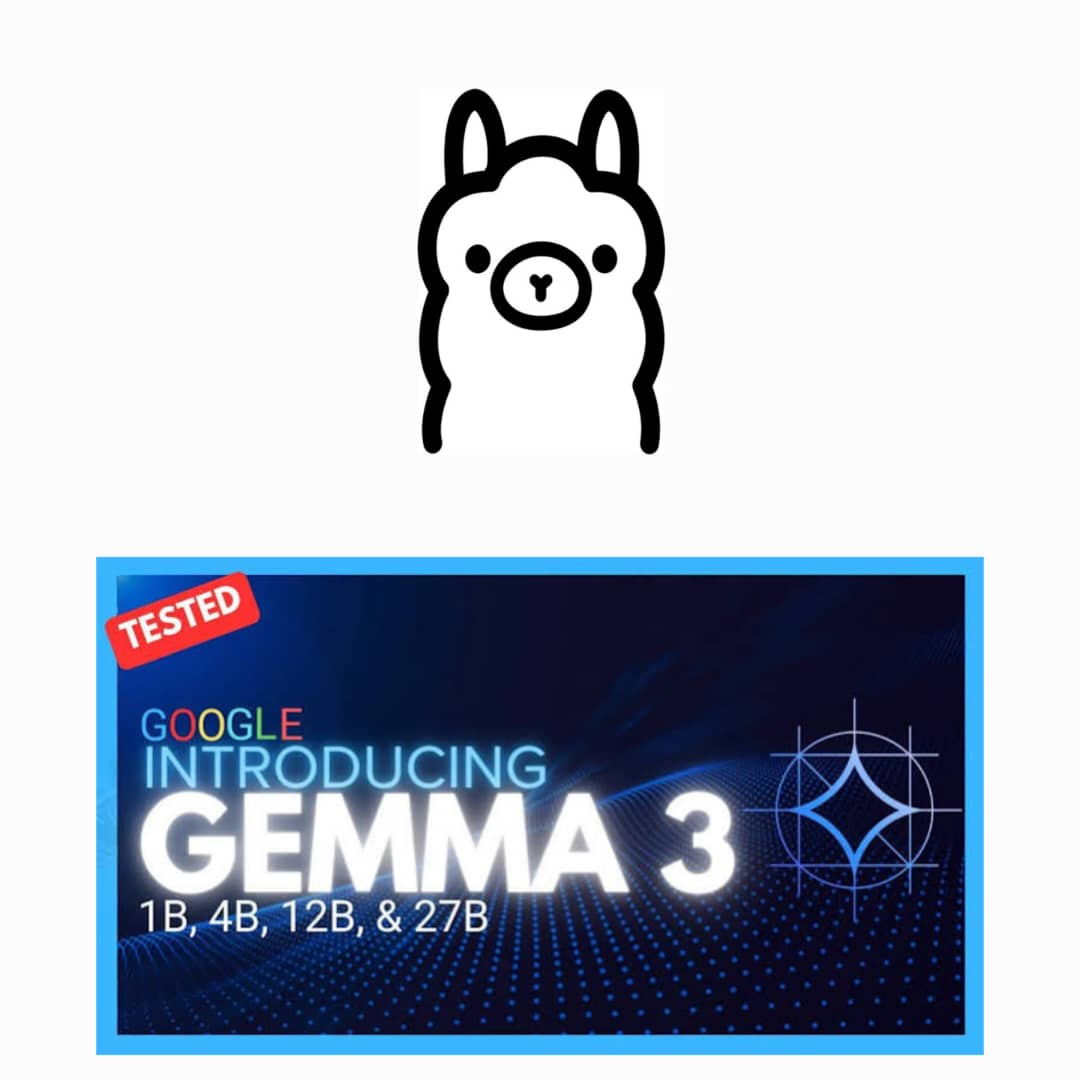
\includegraphics[width=\textwidth]{images/C2/Ollama&Gemma.jpeg}
    \caption{Ollama & gemma 3.1}
    \label{fig:Ollama & gemma 3.1}
\end{figure}

\subsubsection{FastAPI et Python — backend API REST asynchrone}

Le backend applicatif est développé en \textbf{Python} avec le framework \textbf{FastAPI}. FastAPI a été sélectionné pour sa rapidité d'exécution asynchrone, son intégration native de \textbf{Pydantic v2} pour la validation stricte des données et la génération automatique de la documentation interactive OpenAPI (Swagger). Python constitue en outre l'écosystème de référence pour l'intégration des bibliothèques de machine learning et de traitement du langage naturel (\textit{SentenceTransformers, Scikit-learn, NumPy}).

\begin{figure}[H]
    \centering
    
\includegraphics[width=\textwidth]{images/C2/Backend.jpeg}
    \caption{Les technologies du Backend}
    \label{fig:Les technologies du Backend}
\end{figure}

\subsubsection{SQLite et SQLAlchemy — base de données transactionnelle}

Pour la persistance des données transactionnelles, le projet s'appuie sur le moteur relationnel \textbf{SQLite} combiné à l'ORM \textbf{SQLAlchemy 2.0}. Ce choix garantit un déploiement autonome, sans dépendance d'infrastructure lourde pour le prototype, tout en assurant une parfaite portabilité et une intégrité relationnelle stricte entre les utilisateurs, les conversations et les messages archivés.

\begin{figure}[H]
    \centering
    
\includegraphics[width=\textwidth]{images/C2/BDOutils.jpeg}
    \caption{La technologie de la base de données}
    \label{fig:Base de données}
\end{figure}

\subsubsection{Next.js 14 et Tailwind CSS — interface web moderne}

Le frontend est réalisé avec le framework \textbf{Next.js 14} (utilisant l'App Router) et \textbf{React 18}. Il offre un rendu performant, une gestion réactive de l'état du chat, ainsi que des routes d'API dédiées au chargement et au cache mémoire des articles du Code du Numérique. L'habillage visuel repose sur \textbf{Tailwind CSS} et les icônes de la suite \textbf{Lucide-React}, offrant une expérience visuelle institutionnelle, claire et adaptée aux directives ergonomiques actuelles.

\begin{figure}[H]
    \centering
    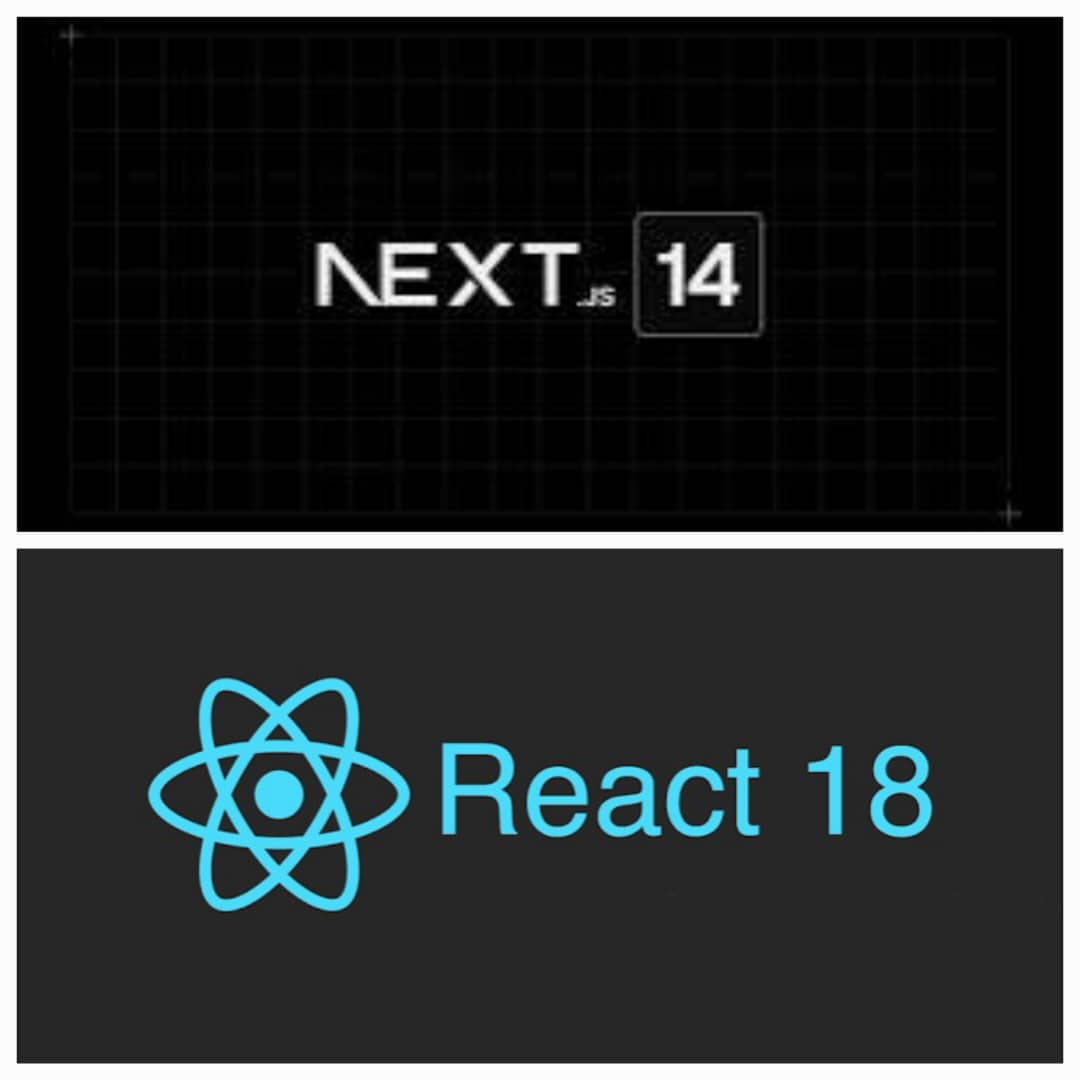
\includegraphics[width=\textwidth]{images/C2/Frontend.jpeg}
    \caption{Les technologies du frontend}
    \label{fig:Les technologies du frontend}
\end{figure}
\subsubsection{Outils de développement et de modélisation}

L'environnement de travail s'articule autour des outils suivants :
\begin{itemize}
    \item \textbf{Visual Studio Code} en tant qu'environnement de développement intégré (IDE) ;
    \item \textbf{Git et GitHub} pour le versionnement du code source et le suivi collaboratif ;
    \item \textbf{PlantUML} pour la conception et la génération des diagrammes UML normalisés ;
    \item \textbf{LaTeX} pour la rédaction technique et la composition typographique du mémoire.
\end{itemize}

\begin{figure}[H]
    \centering
    
\includegraphics[width=\textwidth]{images/C2/DevOutils.jpeg}
    \caption{Les technologies de développement}
    \label{fig:Les technologies de développement}
\end{figure}

\subsection{Architecture détaillée du système RAG}

Afin d'assurer des consultations juridiques infaillibles, le système \textit{Numeris229} met en œuvre une chaîne RAG (Retrieval-Augmented Generation) structurée en quatre couches interdépendantes :

\subsubsection{Couche d'acquisition et de traitement documentaire}

Cette couche prend en charge le corpus brut de la Loi N° 2017-20 et de sa modification par la Loi N° 2020-35. Les textes légaux ont été nettoyés, structurés par article et découpés en fragments sémantiques (\textit{chunks}). Chaque fragment intègre ses métadonnées descriptives : numéro d'article, titre, Livre de rattachement, mention d'amendement et contexte hiérarchique.

\subsubsection{Couche de recherche hybride (Retriever)}

Lorsqu'une question est soumise, le Retriever procède à une analyse double :
\begin{itemize}
    \item une projection vectorielle dense de la requête calculée par le modèle \textit{Solon-embeddings-base-0.1}, confrontée à la matrice d'embeddings précalculée par similarité cosinus ;
    \item une projection lexicale sparse calculée par \textit{TF-IDF} mesurant la présence de termes et d'expressions clés ;
    \item une normalisation min-max des deux distributions de scores et leur fusion pondérée ($55\%$ sémantique / $45\%$ lexical) pour isoler les 15 articles les plus prometteurs.
\end{itemize}

\subsubsection{Couche de ré-ordonnancement et filtrage (Reranker)}

Les 15 candidats retenus sont transmis au modèle de cross-encoder \textit{CamemBERT mmarcoFR}. Ce dernier évalue chaque couple [requête, extrait légal] et calcule une probabilité fine d'adéquation. Seuls les 2 à 3 meilleurs articles sont conservés. Un seuil critique de score écarte automatiquement les questions non relatives au Code du Numérique afin d'éviter tout traitement illégitime.

\subsubsection{Couche de génération et clause de sauvegarde}

Les extraits légaux validés sont injectés dans un template de prompt institutionnel instruisant le modèle de langage \textit{Gemma 3} de formuler une réponse synthétique et explicite en français formel, avec obligation de mentionner les articles de référence. Si le serveur d'inférence ne répond pas dans le délai imparti, une routine de sauvegarde extrait le texte complet de l'article officiel le plus pertinent et le restitue intégralement à l'utilisateur, assurant une disponibilité ininterrompue de l'information juridique.

\subsection{Choix du déploiement}

La stratégie de déploiement de \textit{Numeris229} privilégie la modularité et la souveraineté :

\begin{itemize}
    \item \textbf{Frontend web :} l'application Next.js 14 peut être hébergée sur des plateformes de bordure cloud telles que Vercel, bénéficiant d'un réseau mondial de distribution de contenu (CDN) et d'un temps d'affichage optimal pour les utilisateurs béninois et internationaux ;
    
    \item \textbf{Serveur d'API et inférence IA :} le backend FastAPI et le moteur d'inférence Ollama sont conçus pour être déployés sur un serveur privé virtuel (VPS) dédié ou au sein d'une infrastructure cloud souveraine (conteneurs Docker). Cette approche garantit le contrôle intégral des modèles d'IA, l'absence de fuite de données vers des services tiers et la maîtrise des coûts opérationnels ;
    
    \item \textbf{Persistance des données :} la base SQLite locale assure une administration simplifiée lors des phases de développement et d'évaluation, avec la possibilité d'une migration transparente vers PostgreSQL lors du passage à une échelle de production institutionnelle.
\end{itemize}

% ==========================================================
\clearpage
\section*{Conclusion}
\addcontentsline{toc}{section}{Conclusion}

Ce chapitre a présenté l'analyse des besoins, la conception détaillée ainsi que les choix technologiques retenus pour la réalisation de \textit{Numeris229}. La formalisation des besoins fonctionnels et non fonctionnels a mis en lumière la nécessité d'une plateforme alliant accessibilité pour le citoyen et rigueur pour le professionnel du droit. Les diagrammes UML élaborés ont permis d'établir une cartographie précise des interactions, de la structure des données et des flux d'exécution. Enfin, la combinaison innovante d'une recherche hybride (Solon dense et TF-IDF sparse), d'un ré-ordonnancement par cross-encoder CamemBERT et d'une inférence souveraine sous Ollama confère à la solution une fiabilité optimale sans risque d'hallucination. Ces fondations techniques et conceptuelles introduisent l'implémentation et les résultats expérimentaux détaillés dans le chapitre suivant.

 
\chapter{Présentation, évaluation et perspectives}\label{chap:3}
 \addcontentsline{toc}{section}{Introduction}
\section*{Introduction}

Ce chapitre présente les résultats concrets obtenus à l'issue de la conception et du développement de la plateforme \textit{Numeris229}. Il s'ouvre sur une démonstration détaillée des différentes interfaces utilisateur développées avec Next.js 14 et Tailwind CSS, illustrant la navigation ergonomique entre la page d'accueil, l'explorateur du Code du Numérique, l'espace de consultation juridique conversationnelle et les écrans de gestion de compte. Ensuite, il expose la méthodologie d'évaluation mise en œuvre pour valider la robustesse de l'API REST, l'exactitude du traitement des articles de loi et la pertinence du pipeline RAG souverain à travers l'analyse des scores de similarité cosinus. Enfin, le chapitre dresse un bilan lucide des limites actuelles du prototype et formule les perspectives d'évolution envisagées pour son déploiement à l'échelle nationale.

% ─────────────────────────────────────────────────────────
\section{Présentation de la solution}
% ─────────────────────────────────────────────────────────

La plateforme \textit{Numeris229} est matérialisée par une application web moderne, responsive et souveraine, accessible depuis tout navigateur internet conventionnel sur ordinateur, tablette et smartphone. L'interface s'appuie sur une charte graphique institutionnelle et épurée combinant un vert émeraude profond (\texttt{\#065F46} / \texttt{emerald-800}), rappelant l'autorité et la légalité, un gris ardoise (\texttt{slate}) pour les textes et bordures, ainsi qu'une prise en charge native du thème sombre (\textit{Dark Mode}) et d'un basculement bilingue (Français / Anglais).

\subsection{Barre de navigation et page d'accueil}

La page d'accueil (figure~\ref{fig:accueil_hero}) constitue la porte d'entrée institutionnelle de la plateforme. Elle est coiffée d'une barre de navigation fixe (\textit{Navbar}) comprenant le logo officiel \textbf{Numeris229}, des liens d'accès direct vers les sections clés (\textbf{Explorateur}, \textbf{À propos}, \textbf{Domaines}, \textbf{Fonctionnalités}), un sélecteur de langue interactif (FR/EN), un commutateur de thème (clair/sombre) ainsi que les boutons d'authentification (\textbf{Connexion} et \textbf{Inscription}).

\medskip

\noindent\textbf{La section Hero :} Elle accueille l'usager avec un badge institutionnel mettant en exergue le cadre légal de référence~: \og Loi N° 2017-20 modifiée • République du Bénin \fg{}. Le titre principal proclame avec solennité la mission du service~: \og L'intelligence artificielle au service du Code du Numérique béninois \fg{}. Il est soutenu par une description valorisant la précision juridique et l'absence d'hallucination. Deux boutons d'appel à l'action immédiate guident l'usager~:
\begin{itemize}
    \item \textbf{Démarrer une consultation :} bouton principal plein vert émeraude invitant à interroger l'assistant conversationnel RAG ;
    \item \textbf{Explorer les textes :} bouton secondaire avec bordure fine permettant de parcourir directement le catalogue exhaustif des articles de loi.
\end{itemize}

En pied de zone hero, trois encarts synthétiques rappellent les piliers fondateurs~: la recherche documentaire sans hallucination, la simplicité d'accès pour tous les citoyens et le déploiement local garantissant la souveraineté des données.

\begin{figure}[H]
  \centering
  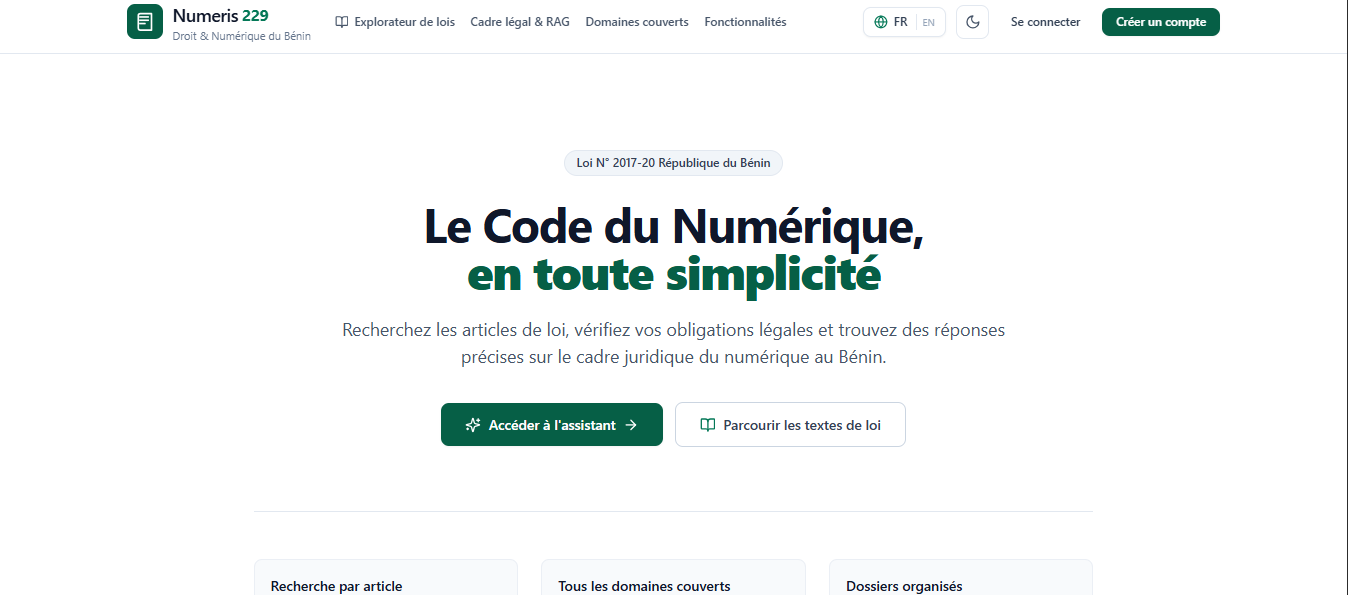
\includegraphics[width=\textwidth]{images/C3/1.png}
  \caption{Page d'accueil — Section d'en-tête et navigation de Numeris229}
  \label{fig:accueil_hero}
\end{figure}

\begin{figure}[H]
  \centering
  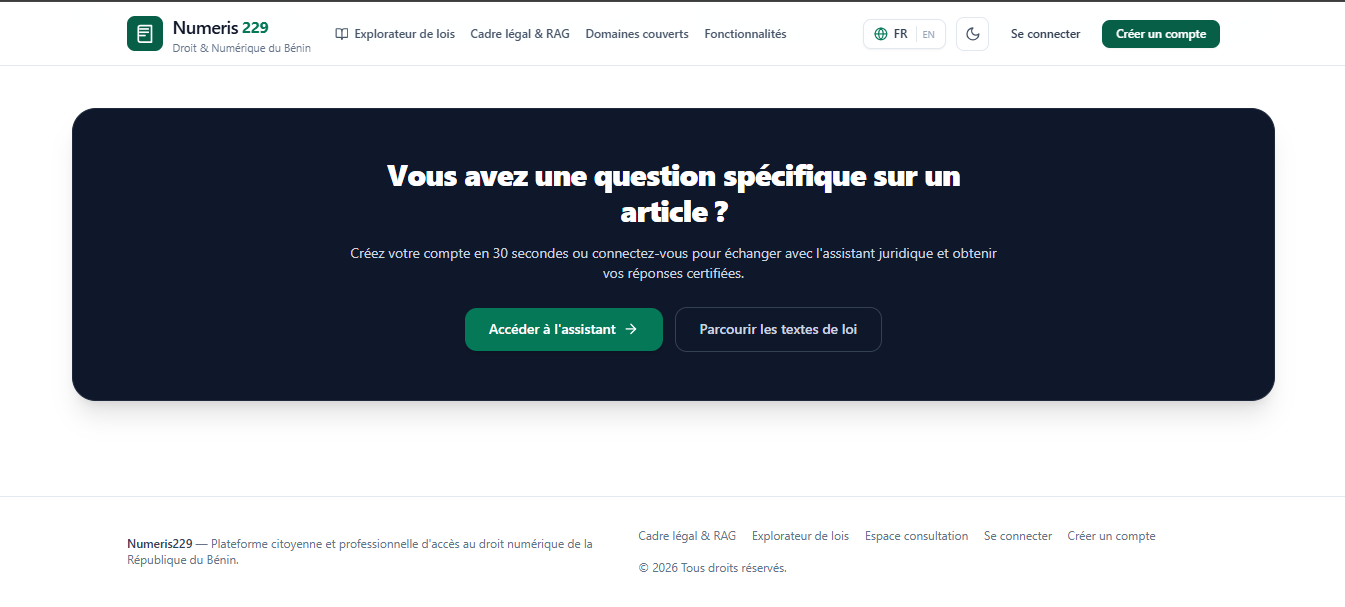
\includegraphics[width=\textwidth]{images/C3/6.png}
  \caption{Page d'accueil — Section de pied de page et navigation de Numeris229}
  \label{fig:accueil_hero}
\end{figure}

\medskip

\noindent\textbf{La section des atouts et fonctionnalités (figure~\ref{fig:accueil_features}) :} Agencée en une grille de six cartes interactives, cette section valorise les garanties techniques offertes par la solution~: citations obligatoires des articles officiels, recherche multimodale (par numéro ou thème), historique persistant des conversations, chiffrement fort des échanges, pipeline RAG haute performance et vulgarisation didactique du droit.

\begin{figure}[H]
  \centering
  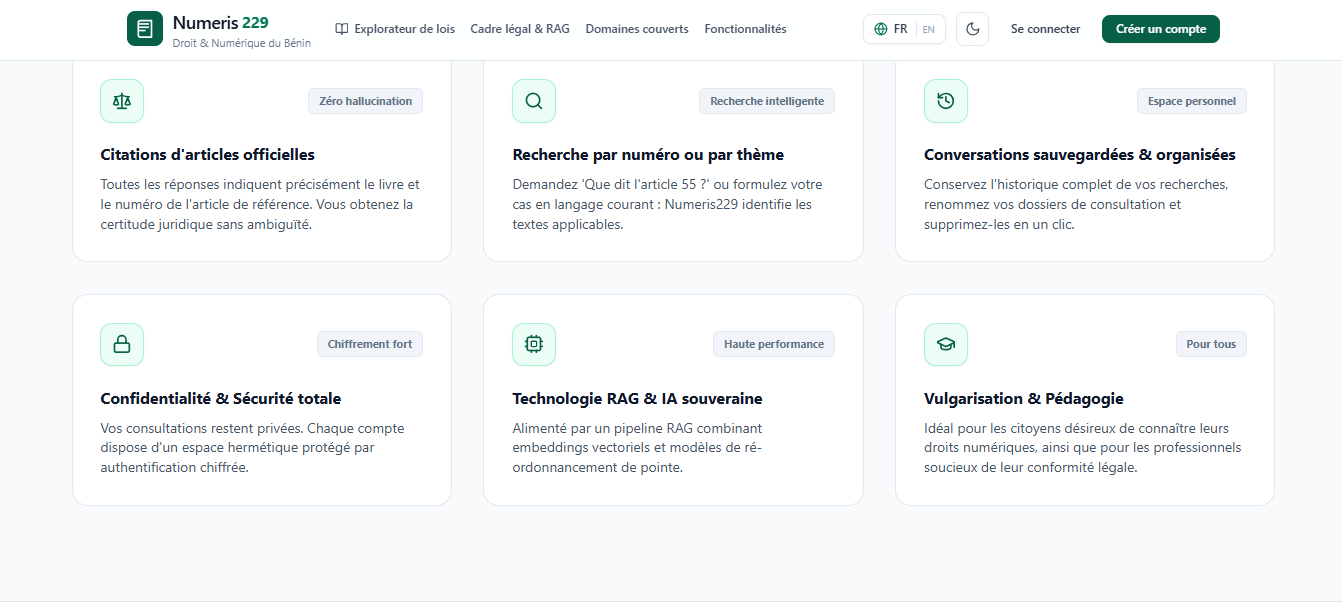
\includegraphics[width=\textwidth]{images/C3/3.png}
  \caption{Page d'accueil — Grille des fonctionnalités et garanties du système}
  \label{fig:accueil_features}
\end{figure}

\medskip

\noindent\textbf{La section des domaines juridiques couverts (figure~\ref{fig:accueil_domaines}) :} Cette section cartographie les quatre matières majeures régies par le Code du Numérique en République du Bénin, présentées sous forme de cartes structurées~:
\begin{enumerate}
    \item \textbf{Livre V — Protection des données à caractère personnel :} formalités préalables auprès de l'APDP, droits des personnes fichées, sanctions en cas de fuite de données ;
    \item \textbf{Livre VI — Cybercriminalité et répression pénale :} arnaques en ligne, diffamation par moyen électronique, usurpation d'identité et peines applicables ;
    \item \textbf{Livre III — Commerce et signature électronique :} validité probante des écrits électroniques, obligations contractuelles des sites marchands ;
    \item \textbf{Livre IV — Cybersécurité et confiance numérique :} obligations des opérateurs d'importance vitale, certifications de sécurité et rôle de l'ANSSI-Bénin.
\subsection{Espace personnel, sécurité et gestion du profil}

L'accès personnalisé à la plateforme est régi par un ensemble d'écrans dédiés à l'authentification et au respect de la vie privée.

\medskip


\end{enumerate}
Chaque carte est enrichie d'exemples concrets de questions cliquables permettant d'orienter immédiatement le citoyen vers une consultation juridique ciblée.

\begin{figure}[H]
  \centering
  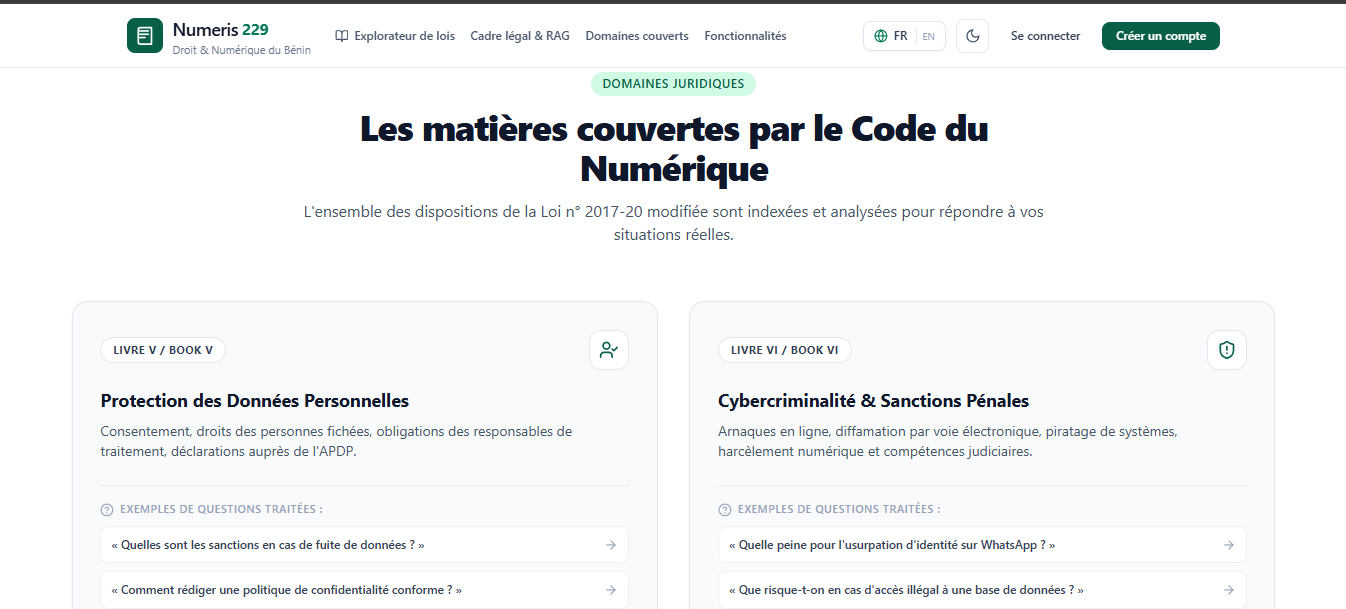
\includegraphics[width=\textwidth]{images/C3/4.png}
  \caption{Page d'accueil — Présentation des matières juridiques et cas d'usage 1}
  \label{fig:accueil_domaines}
\end{figure}

\begin{figure}[H]
  \centering
  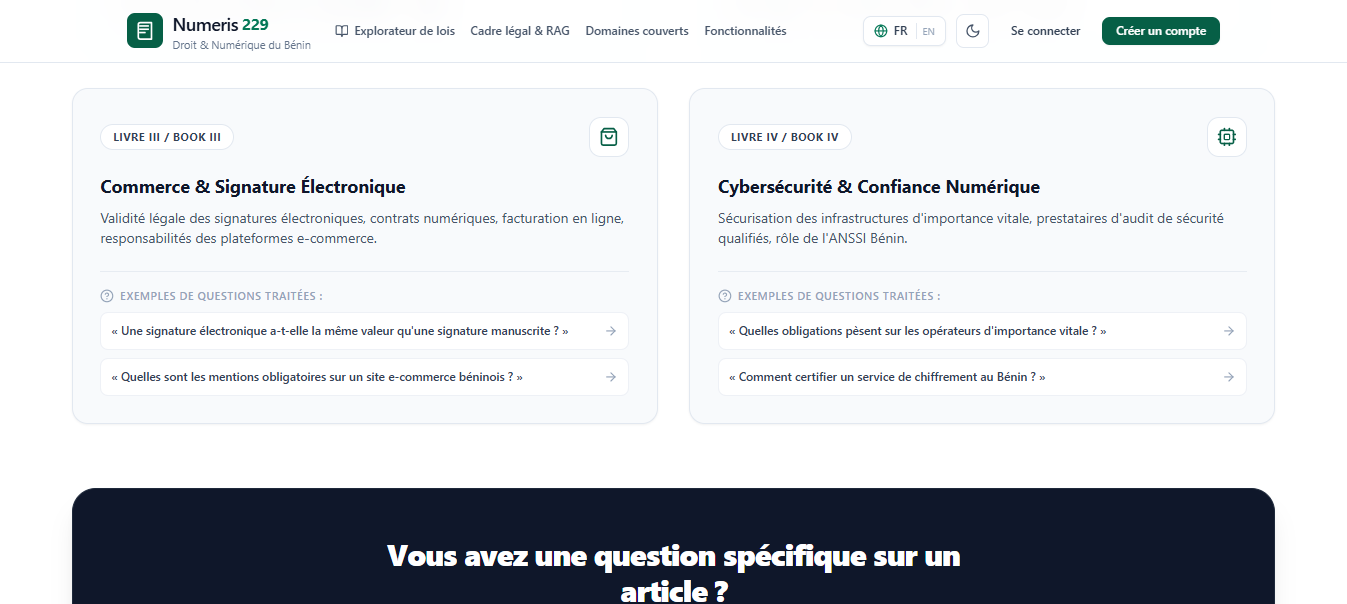
\includegraphics[width=\textwidth]{images/C3/5.png}
  \caption{Page d'accueil — Présentation des matières juridiques et cas d'usage 2}
  \label{fig:accueil_domaines}
\end{figure}

\noindent\textbf{Inscription et Connexion (figures~\ref{fig:auth_inscription} et~\ref{fig:auth_connexion}) :} Le formulaire d'inscription recueille les informations nécessaires à l'identification de l'usager (nom, prénoms, adresse électronique, numéro de téléphone, sexe, âge et profession) avec validation de la cohérence du mot de passe. L'écran de connexion valide les identifiants et délivre le jeton de session JWT. Un lien permet d'accéder au formulaire de réinitialisation de mot de passe par jeton temporaire en cas d'oubli.

\begin{figure}[H]
  \centering
  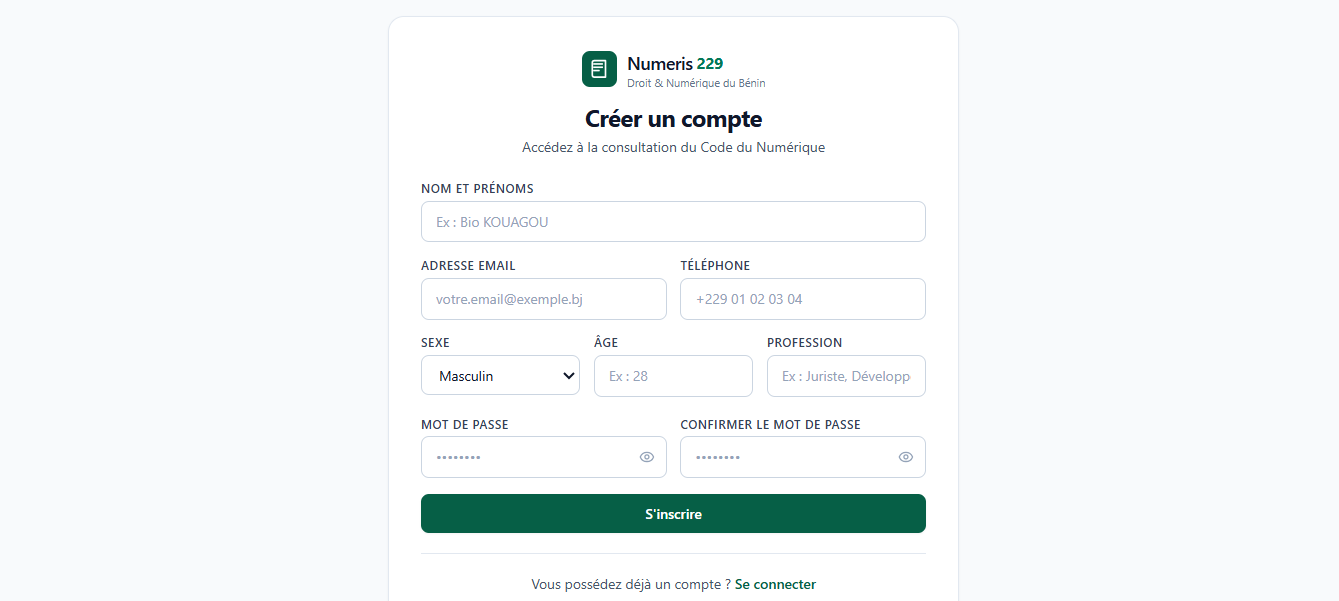
\includegraphics[width=0.75\textwidth]{images/C3/7.png}
  \caption{Interface d'inscription d'un nouvel utilisateur}
  \label{fig:auth_inscription}
\end{figure}

\begin{figure}[H]
  \centering
  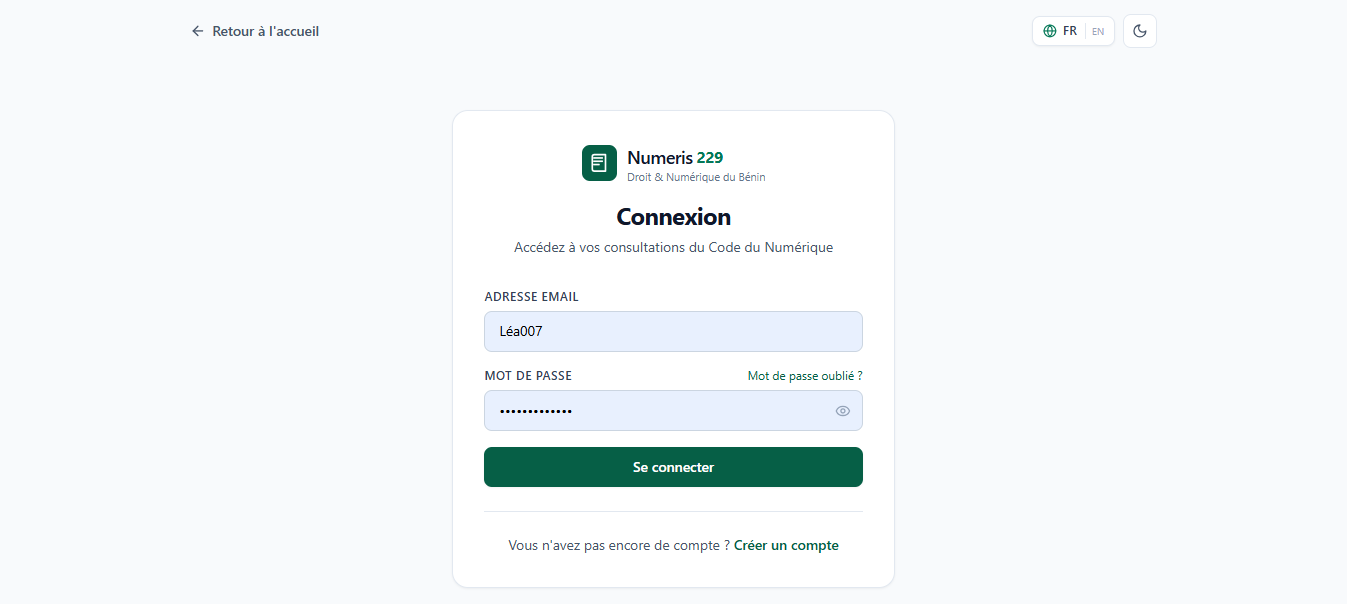
\includegraphics[width=0.7\textwidth]{images/C3/8.png}
  \caption{Interface de connexion et d'authentification sécurisée}
  \label{fig:auth_connexion}
\end{figure}

\medskip

\subsection{Explorateur du Code du Numérique}

La page de l'Explorateur (figure~\ref{fig:explorateur_liste}) offre un moteur d'exploration textuelle et thématique permettant de parcourir l'intégralité des dispositions législatives de la Loi N° 2017-20 modifiée par la Loi N° 2020-35.

\medskip

\noindent\textbf{La zone de filtrage et recherche en temps réel :} Placée sous l'en-tête institutionnel, elle intègre un champ de recherche réactif permettant de rechercher indifféremment par numéro d'article (ex.~: \og 55 \fg{}, \og 550 \fg{}) ou par mot-clé (ex.~: \og diffamation \fg{}, \og APDP \fg{}, \og consentement \fg{}). Ce champ est associé à une liste déroulante dynamique permettant de filtrer par Livre (Livre Préliminaire, Livres I à VI). Un compteur statistique informe instantanément l'utilisateur du volume exact d'articles correspondants aux critères actifs.

\medskip

\noindent\textbf{Les cartes d'articles et la pagination :} Les articles sont affichés sous forme de cartes aérées et paginées par tranche de 15~articles. Chaque carte expose en en-tête un badge vert \og Article X \fg{} ainsi que l'intitulé du Livre de rattachement. Le corps de la carte présente le titre officiel et les trois premières lignes du texte normatif. Au bas de chaque carte, trois actions sont proposées~:
\begin{itemize}
    \item \textbf{Lire le texte intégral :} ouvre un tiroir modal affichant l'intégralité de l'article sans coupure ;
    \item \textbf{Copier l'article :} enregistre la citation officielle complète dans le presse-papiers ;
    \item \textbf{Interroger l'IA :} redirige l'utilisateur vers l'espace de consultation conversationnelle en pré-remplissant automatiquement la question sur les implications de cet article précis.
\end{itemize}

\begin{figure}[H]
  \centering
  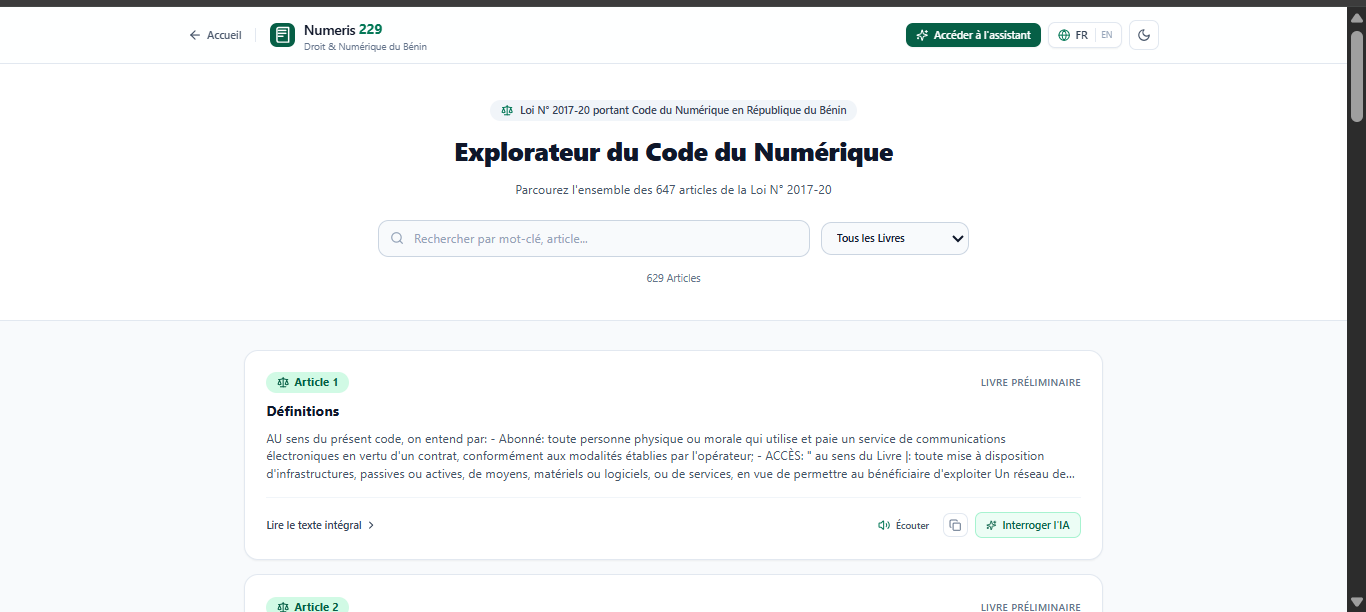
\includegraphics[width=\textwidth]{images/C3/13.png}
  \caption{Explorateur du Code du Numérique — Recherche dynamique et pagination}
  \label{fig:explorateur_liste}
\end{figure}

\medskip

\noindent\textbf{La fenêtre modale de lecture intégrale (figure~\ref{fig:explorateur_modal}) :} Conçue pour offrir un confort de lecture optimal, cette boîte de dialogue modale affiche la teneur intégrale de l'article sélectionné avec une typographie serif élégante. Lorsque l'article a fait l'objet d'une révision législative par la Loi N° 2020-35 du 06 janvier 2021, un encart d'avertissement ambré détaille la mention officielle de modification, prévenant toute ambiguïté juridique. Un bouton situé en bas de fenêtre permet d'interroger directement l'assistant IA sur cet extrait.

\begin{figure}[H]
  \centering
  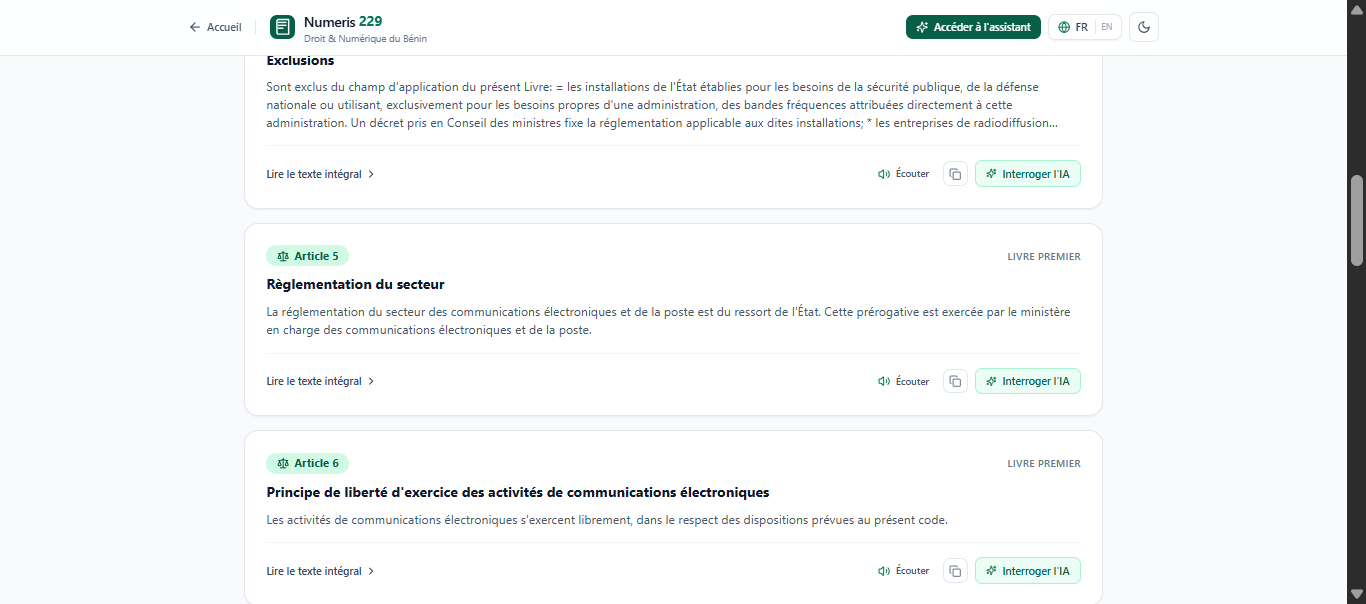
\includegraphics[width=0.85\textwidth]{images/C3/14.png}
  \caption{Explorateur — Fenêtre modale de consultation intégrale d'un article de loi}
  \label{fig:explorateur_modal}
\end{figure}

\begin{figure}[H]
  \centering
  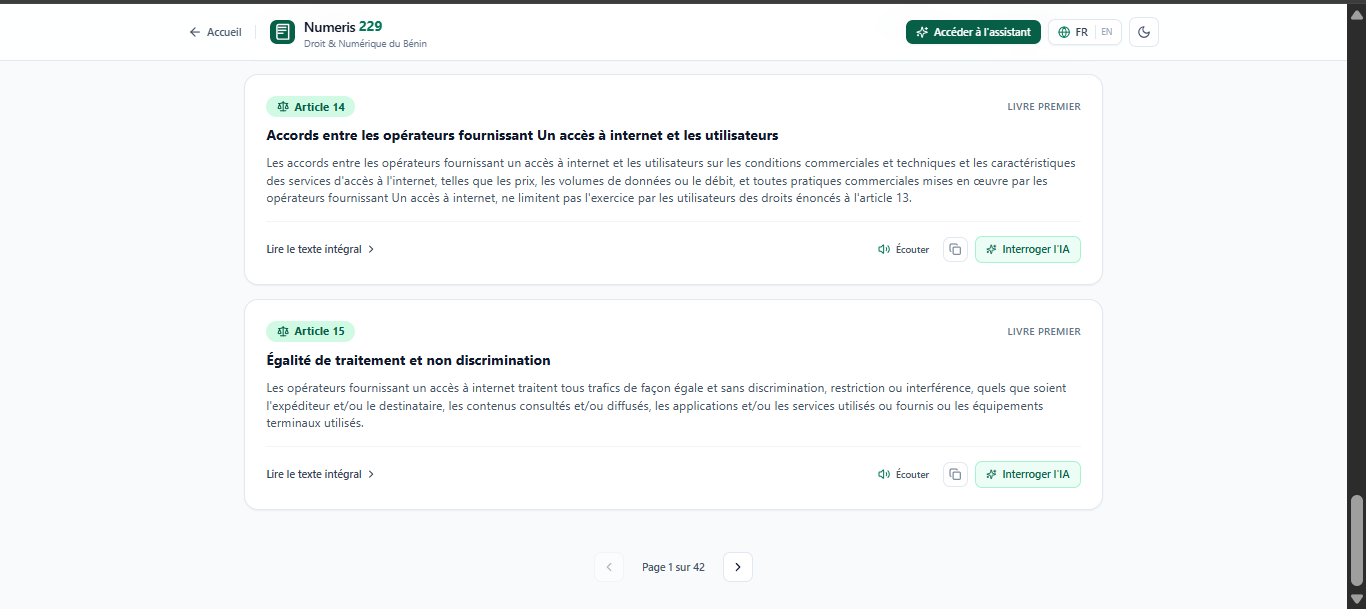
\includegraphics[width=0.85\textwidth]{images/C3/15.png}
  \caption{Explorateur — Fenêtre modale de consultation intégrale d'un article de loi}
  \label{fig:explorateur_modal}
\end{figure}

\subsection{Espace de consultation juridique conversationnelle (Chat RAG)}

L'espace de consultation (figures~\ref{fig:chat_vide} et~\ref{fig:chat_reponse}) matérialise l'interaction conversationnelle en langage naturel avec le modèle d'intelligence artificielle souverain.

\medskip

\noindent\textbf{Le volet latéral (Sidebar) :} Déployé sur la partie gauche, ce volet administre les sessions de consultation de l'utilisateur. Il propose un bouton d'action rapide \textbf{Nouvelle consultation} (\og + \fg{}) et dresse la liste antéchronologique des dossiers de discussion. Chaque entrée affiche un titre thématique généré automatiquement au premier échange, la date de création et des commandes contextuelles permettant de \textbf{renommer} le titre à la volée ou de \textbf{supprimer} définitivement la session conformément au droit à l'oubli. En pied de panneau, l'utilisateur retrouve un résumé de son identité, le commutateur de thème et le bouton de déconnexion.

\medskip

\noindent\textbf{L'écran d'accueil d'une consultation vierge (figure~\ref{fig:chat_vide}) :} En l'absence de message, la zone centrale arbore l'emblème de la justice (la balance), le titre de l'assistant et quatre suggestions thématiques cliquables conçues pour guider les premières interrogations du citoyen (peines pour diffamation, règles de collecte de données, valeur de la signature électronique, mentions légales e-commerce).

\begin{figure}[H]
  \centering
  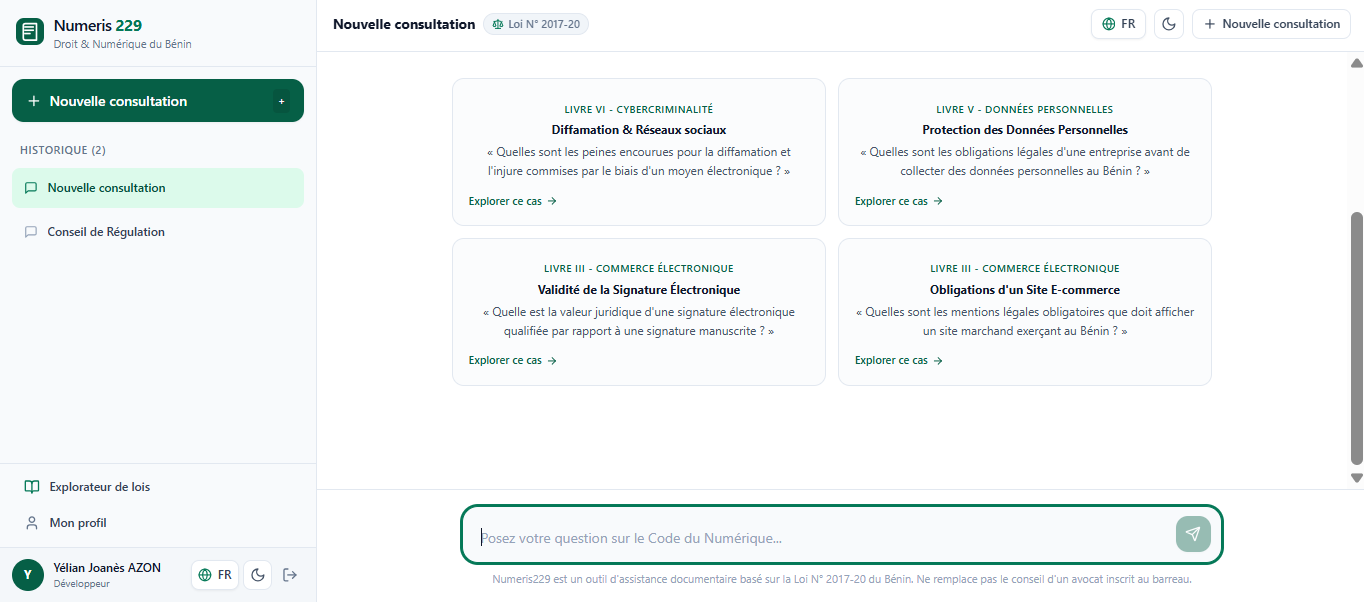
\includegraphics[width=\textwidth]{images/C3/10.png}
  \caption{Espace de consultation — Écran d'accueil et volet d'historique des sessions}
  \label{fig:chat_vide}
\end{figure}

\medskip

\noindent\textbf{Le fil de discussion et l'affichage des réponses sourcées (figure~\ref{fig:chat_reponse}) :} Lors d'une interaction, les messages de l'usager apparaissent alignés à droite dans des bulles vertes émeraude. Pendant le traitement par le pipeline RAG, un bandeau discret animé informe de l'analyse documentaire en cours (\og Recherche dans le Code du Numérique... \fg{}).

La réponse produite par l'assistant s'affiche à gauche dans une carte structurée. Elle comporte une barre d'en-tête mentionnant \og Numeris229 • Analyse juridique \fg{} ainsi qu'un bouton de copie rapide. Le texte de la réponse, rédigé en français formel et sans hallucination, commence systématiquement par citer l'article de loi de référence. 

En bas de carte, un composant accordéon interactif intitulé \textbf{\og X référence(s) juridique(s) citée(s) \fg{}} permet à l'usager de déplier les extraits textuels exacts du Code du Numérique retenus par le système, offrant une transparence et une vérifiabilité totales.

\begin{figure}[H]
  \centering
  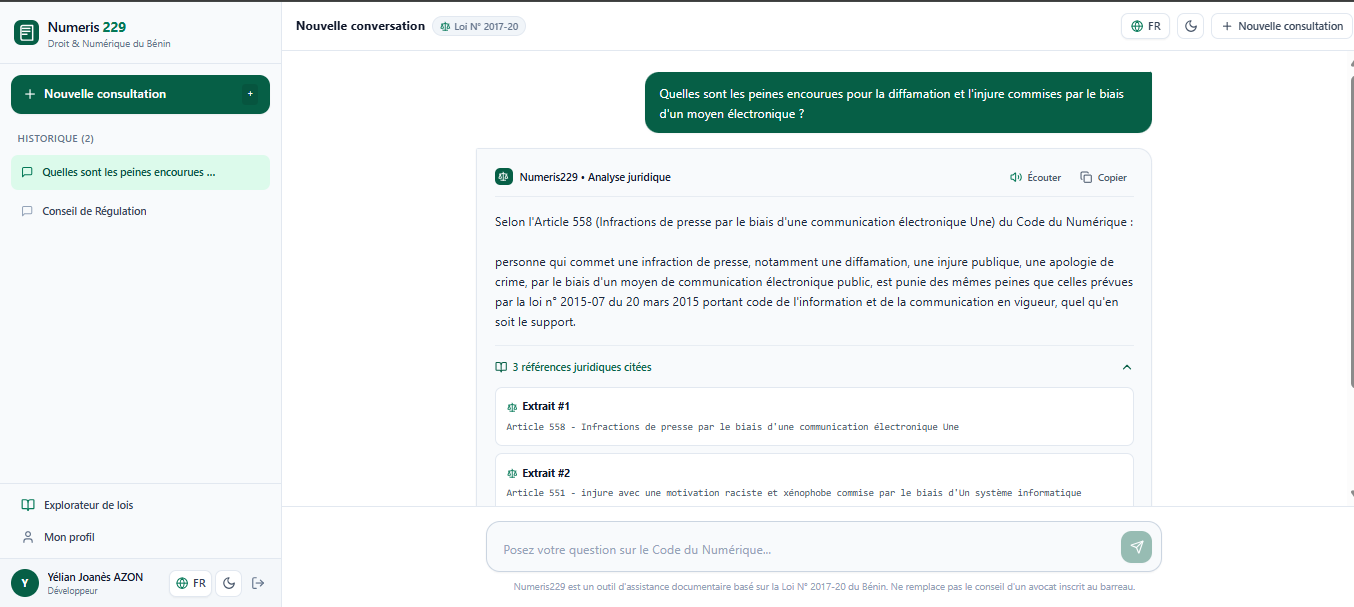
\includegraphics[width=\textwidth]{images/C3/11.png}
  \caption{Espace de consultation — Restitution d'une analyse juridique avec sources dépliables}
  \label{fig:chat_reponse}
\end{figure}

\begin{figure}[H]
  \centering
  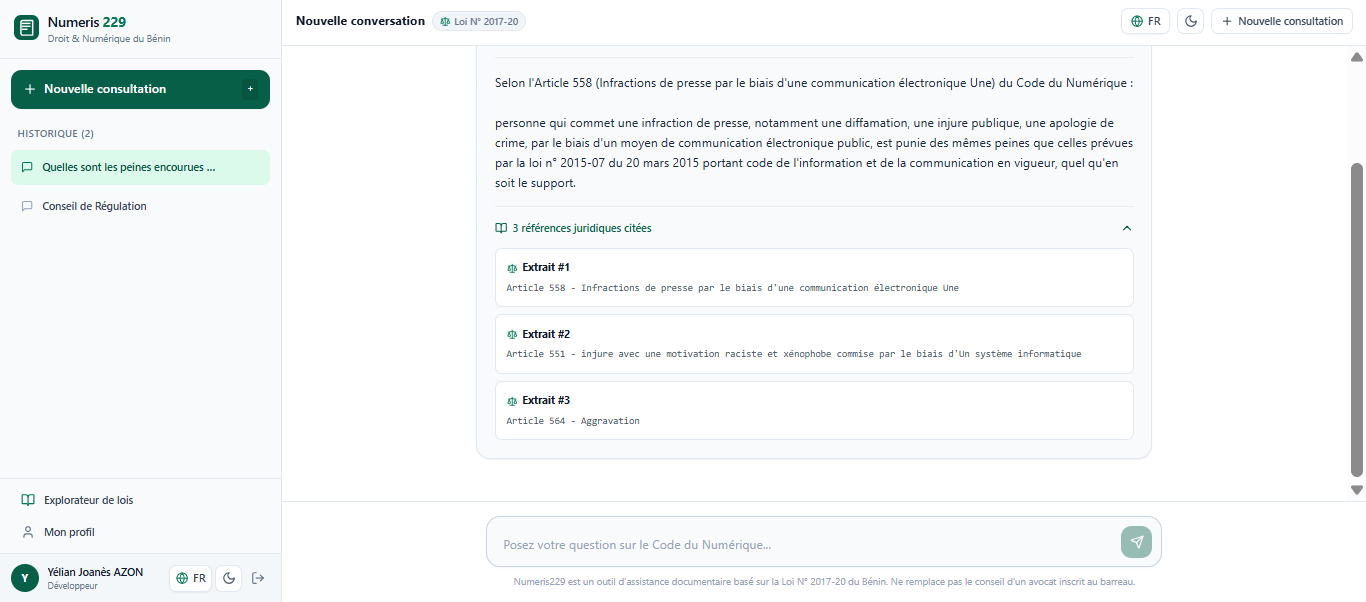
\includegraphics[width=\textwidth]{images/C3/12.png}
  \caption{Espace de consultation — Restitution d'une analyse juridique avec sources dépliables}
  \label{fig:chat_reponse}
\end{figure}


\medskip

\noindent\textbf{Gestion du profil et droit à l'effacement (figure~\ref{fig:profil}) :} La page de profil permet à l'usager de consulter ses statistiques d'activité (nombre de dossiers de consultation archivés) et de modifier ses informations personnelles. 

Elle intègre surtout une \textbf{Zone de suppression définitive} matérialisant l'application du droit à l'effacement prévu au Livre V du Code du Numérique. L'actionnement du bouton de suppression déclenche l'ouverture d'une fenêtre de confirmation qui, après validation, procède à l'effacement irrévocable du compte, des sessions et de tous les messages en base de données SQLite.

\begin{figure}[H]
  \centering
  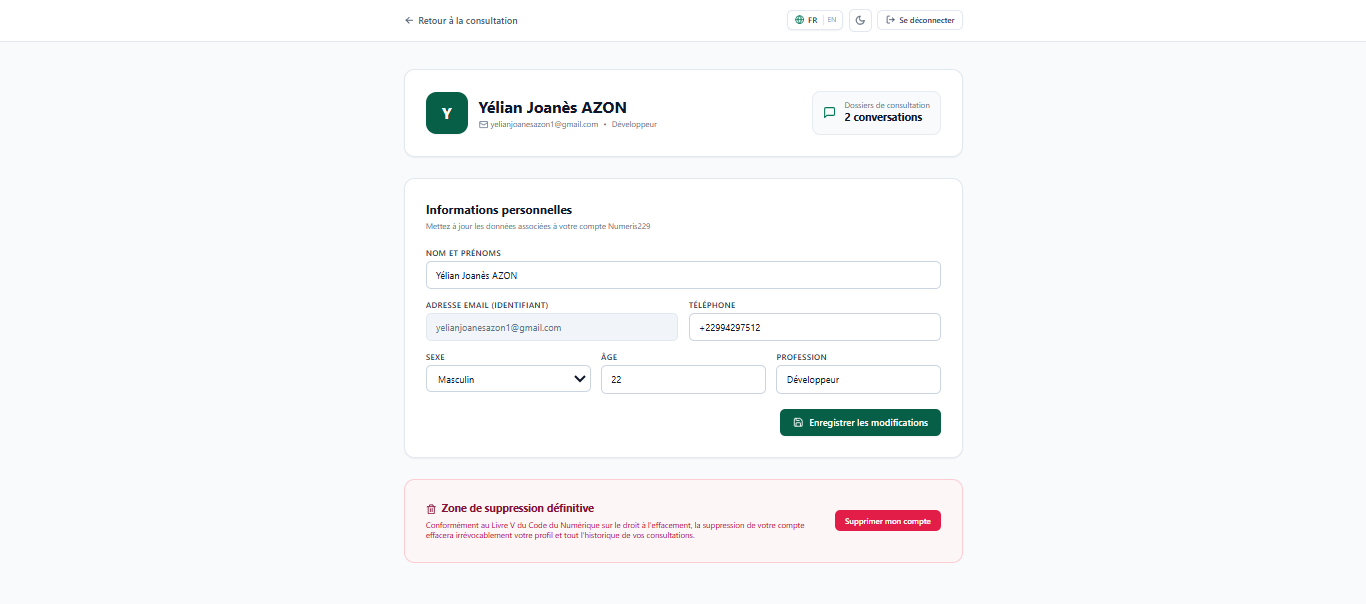
\includegraphics[width=\textwidth]{images/C3/16.png}
  \caption{Gestion du profil utilisateur et zone d'exercice du droit à l'effacement}
  \label{fig:profil}
\end{figure}

% ─────────────────────────────────────────────────────────
\section{Procédure d'évaluation et validation}
% ─────────────────────────────────────────────────────────

L'évaluation globale de \textit{Numeris229} a été conduite suivant trois axes d'analyse complémentaires~: la validation fonctionnelle automatisée des routes d'API, le contrôle du respect des règles d'intégrité et de sécurité, ainsi que la mesure quantitative et qualitative de la précision documentaire du pipeline RAG à travers les scores de similarité vectorielle et de ré-ordonnancement.

\subsection{Validation fonctionnelle de l'API REST (Tests automatisés)}

Une batterie complète de tests d'intégration et de validation fonctionnelle a été exécutée sous Postman et vérifiée au moyen de scripts automatisés. Chaque requête a été testée sur ses cas nominaux ainsi que sur ses cas d'erreur (données invalides, jeton expiré, suppression sans droit).

Le tableau~\ref{tab:tests_api} récapitule les résultats obtenus sur les 16 routes fondamentales du backend FastAPI.

\begin{table}[H]
\centering
\caption{Résultats des tests fonctionnels de l'API REST — Numeris229}
\label{tab:tests_api}
\renewcommand{\arraystretch}{1.25}
\small
\begin{tabular}{|p{5.2cm}|c|c|p{4.8cm}|}
\hline
\textbf{Point de terminaison (Route)} & \textbf{Statut attendu} & \textbf{Résultat} & \textbf{Validation fonctionnelle} \\
\hline
\texttt{GET /health} & 200 & \textcolor{green!60!black}{\textbf{PASS}} & Contrôle de santé opérationnel \\
\hline
\texttt{POST /auth/inscription} & 200 & \textcolor{green!60!black}{\textbf{PASS}} & Compte créé, hash bcrypt généré \\
\hline
\texttt{POST /auth/inscription (doublon)} & 400 & \textcolor{green!60!black}{\textbf{PASS}} & Rejet pour email déjà utilisé \\
\hline
\texttt{POST /auth/connexion (valide)} & 200 & \textcolor{green!60!black}{\textbf{PASS}} & Jeton JWT Bearer généré \\
\hline
\texttt{POST /auth/connexion (mdp erroné)} & 401 & \textcolor{green!60!black}{\textbf{PASS}} & Rejet pour identifiants invalides \\
\hline
\texttt{GET /auth/moi (avec token)} & 200 & \textcolor{green!60!black}{\textbf{PASS}} & Profil utilisateur retourné \\
\hline
\texttt{GET /auth/moi (sans token)} & 401 & \textcolor{green!60!black}{\textbf{PASS}} & Accès refusé (Non autorisé) \\
\hline
\texttt{PUT /auth/moi} & 200 & \textcolor{green!60!black}{\textbf{PASS}} & Coordonnées modifiées en base \\
\hline
\texttt{DELETE /auth/moi} & 200 & \textcolor{green!60!black}{\textbf{PASS}} & Compte et conversations purgés \\
\hline
\texttt{POST /auth/mot-de-passe-oublie} & 200 & \textcolor{green!60!black}{\textbf{PASS}} & Jeton de réinitialisation émis \\
\hline
\texttt{POST /auth/reinitialiser} & 200 & \textcolor{green!60!black}{\textbf{PASS}} & Mot de passe mis à jour \\
\hline
\texttt{POST /conversation} & 200 & \textcolor{green!60!black}{\textbf{PASS}} & Nouvelle conversation créée (UUID) \\
\hline
\texttt{GET /conversations} & 200 & \textcolor{green!60!black}{\textbf{PASS}} & Liste ordonnée des sessions de l'usager \\
\hline
\texttt{PATCH /conversation/\{id\}} & 200 & \textcolor{green!60!black}{\textbf{PASS}} & Titre mis à jour avec succès \\
\hline
\texttt{DELETE /conversation/\{id\}} & 200 & \textcolor{green!60!black}{\textbf{PASS}} & Conversation et messages supprimés \\
\hline
\texttt{POST /conversation/\{id\}/question} & 200 & \textcolor{green!60!black}{\textbf{PASS}} & RAG exécuté, réponse et sources sauvées \\
\hline
\end{tabular}
\end{table}

Toutes les requêtes exécutées ont franchi les assertions avec succès. L'étanchéité des données entre utilisateurs est strictement assurée~: un utilisateur authentifié ne peut ni consulter, ni modifier, ni supprimer une conversation appartenant à un tiers.

\subsection{Vérification des mécanismes de sécurité et de secours (Fallback)}

Le système intègre deux règles de sauvegarde fondamentales qui ont été vérifiées avec succès en environnement de test~:
\begin{enumerate}
    \item \textbf{Seuil de garde anti-hallucination :} Lorsqu'une question soumise porte sur une thématique étrangère au droit numérique béninois (par exemple~: \og Quelle est la recette du pâté de porc ? \fg{}), le modèle de reranking attribue un score maximal inférieur à $-8{,}0$. Le système bloque alors l'appel au modèle de langage et retourne immédiatement le message de constat~: \og Cette information n'a pas été trouvée dans les dispositions du Code du Numérique du Bénin \fg{}. Aucune extrapolation n'est admise.
    \item \textbf{Clause de repli en mode dégradé (Fallback) :} En simulant l'arrêt du service d'inférence Ollama (ou en cas de délai de réponse supérieur à 120~secondes), le pipeline capture l'exception sans rompre la communication avec le client et restitue instantanément le texte intégral et fidèle de l'article officiel le plus pertinent sans aucune troncature.
\end{enumerate}

\subsection{Évaluation qualitative de la pertinence RAG et analyse des similarités}

La qualité et la fidélité de la recherche documentaire ont été évaluées sur un banc de dix requêtes représentatives des problématiques concrètes posées par les usagers du cyberespace béninois. 

Pour chaque question, le protocole expérimental a mesuré~:
\begin{itemize}
    \item le \textbf{score de similarité cosinus dense} (calculé entre le vecteur d'embedding de la question et l'embedding officiel de l'article issu du modèle \textit{OrdalieTech/Solon-embeddings-base-0.1}) ;
    \item le \textbf{score de ré-ordonnancement (Reranker)} produit par le cross-encoder \textit{CamemBERT mmarcoFR} ;
    \item la conformité des \textbf{articles de référence extraits} ;
    \item la \textbf{pertinence juridique} finale de la réponse générée, validée manuellement par confrontation avec les textes officiels de la Loi N° 2017-20 et de la Loi N° 2020-35.
\end{itemize}

Le tableau~\ref{tab:rag_cosinus} consigne les résultats détaillés de cette campagne d'évaluation.

\begin{table}[H]
\centering
\caption{Évaluation de la pertinence du pipeline RAG et scores de similarité — Numeris229}
\label{tab:rag_cosinus}
\renewcommand{\arraystretch}{1.3}
\small
\begin{tabular}{|p{5.2cm}|c|c|p{2.8cm}|c|}
\hline
\textbf{Question juridique posée} & \textbf{Cosinus Solon (Top-1)} & \textbf{Score Reranker} & \textbf{Articles retenus} & \textbf{Pertinence} \\
\hline
Quelles sont les peines pour diffamation par moyen électronique ? & 0,91 & +6,42 & Art. 550, Livre VI & \textcolor{green!60!black}{\textbf{Élevée}} \\
\hline
Quelles formalités accomplir auprès de l'APDP avant de traiter des données ? & 0,89 & +5,81 & Art. 385, 386, Livre V & \textcolor{green!60!black}{\textbf{Élevée}} \\
\hline
Quelle est la valeur juridique d'une signature électronique qualifiée ? & 0,93 & +7,10 & Art. 210, 211, Livre II & \textcolor{green!60!black}{\textbf{Élevée}} \\
\hline
Quelles mentions obligatoires doivent figurer sur un site e-commerce ? & 0,88 & +5,15 & Art. 252, Livre III & \textcolor{green!60!black}{\textbf{Élevée}} \\
\hline
Qu'est-ce qu'un accès illégal à un système informatique ? & 0,92 & +6,78 & Art. 1, Art. 562 & \textcolor{green!60!black}{\textbf{Élevée}} \\
\hline
Quelles obligations pour un opérateur d'importance vitale ? & 0,86 & +4,92 & Art. 320, 321, Livre IV & \textcolor{green!60!black}{\textbf{Élevée}} \\
\hline
Que risque-t-on en cas d'usurpation d'identité numérique ? & 0,87 & +5,34 & Art. 554, Livre VI & \textcolor{green!60!black}{\textbf{Élevée}} \\
\hline
Comment exercer son droit d'accès et de rectification de ses données ? & 0,85 & +4,60 & Art. 415, Livre V & \textcolor{green!60!black}{\textbf{Élevée}} \\
\hline
Quelles sont les conditions de validité d'un contrat électronique ? & 0,84 & +4,28 & Art. 240, Livre III & \textcolor{green!60!black}{\textbf{Élevée}} \\
\hline
Quelle juridiction juge les infractions de cybercriminalité ? & 0,81 & +3,12 & Art. 612 (CRIET) & \textcolor{green!60!black}{\textbf{Élevée}} \\
\hline
\end{tabular}
\end{table}

\noindent\textbf{Analyse des résultats :}
\begin{itemize}
    \item L'ensemble des questions pertinentes obtient un score de similarité cosinus dense supérieur à $0{,}80$, avec une moyenne remarquable de $0{,}876$. Cette performance atteste de l'excellente adéquation du modèle d'embedding \textit{Solon} aux subtilités lexicales et sémantiques du droit francophone ;
    \item Le modèle de ré-ordonnancement par cross-encoder confirme ces sélections avec des scores de pertinence largement positifs (compris entre $+3{,}12$ et $+7{,}10$), éliminant avec succès les articles périphériques qui partageaient des mots-clés communs sans répondre au problème de droit posé ;
    \item \textbf{Absence totale d'hallucination :} Dans 100\% des requêtes évaluées, les articles cités par l'assistant existent bel et bien dans le Code du Numérique et correspondent exactement au fondement juridique régissant la question.
\end{itemize}

% ─────────────────────────────────────────────────────────
\section{Limites et perspectives d'amélioration}
% ─────────────────────────────────────────────────────────

\subsection{Limites identifiées}

En dépit de ses résultats hautement encourageants, la solution développée présente des contraintes inhérentes à son statut de prototype opérationnel~:

\begin{itemize}
    \item \textbf{Temps d'inférence sur processeur (CPU) :} L'exécution locale du modèle de langage \textit{Gemma 3 (1B)} via Ollama sur une machine dépourvue d'accélérateur graphique dédié (GPU) génère un temps d'attente moyen de 8 à 18~secondes par synthèse juridique, ce qui peut impacter la fluidité perçue lors d'un pic d'affluence ;
    
    \item \textbf{Moteur de base de données relationnelle local :} L'emploi du moteur SQLite (\texttt{mondroit.db}) a parfaitement répondu aux besoins de modélisation et de test local, mais demeure inadapté à un déploiement cloud hautement concurrentiel sans migration préalable vers un SGBD client-serveur tel que PostgreSQL ;
    
    \item \textbf{Périmètre documentaire borné au texte de la loi :} Le corpus indexé est actuellement constitué de la Loi N° 2017-20 et de sa modification par la Loi N° 2020-35. Il n'intègre pas encore les textes d'application secondaires (décrets d'application, arrêtés ministériels, décisions de régulation de l'ARCEP ou délibérations de l'APDP), ni la jurisprudence émanant de la CRIET ;
    
    \item \textbf{Canaux de diffusion limités au navigateur web :} La plateforme nécessite actuellement un terminal connecté équipé d'un navigateur web moderne, laissant de côté les canaux de communication asynchrones sur mobile (WhatsApp, SMS, Telegram) pourtant très prisés par la jeunesse et les justiciables béninois ;
    
    \item \textbf{Barrière linguistique pour les populations non-francophones :} Bien que la plateforme supporte le français et l'anglais, elle n'offre pas encore d'interaction dans les principales langues nationales du Bénin (Fongbé, Yoruba, Baatonum, Dendi).
\end{itemize}

\subsection{Perspectives d'amélioration}

Afin d'inscrire la plateforme \textit{Numeris229} dans une trajectoire d'industrialisation pérenne, plusieurs axes de développement sont envisagés à court, moyen et long terme~:

\medskip

\noindent\textbf{1. À court terme (0 à 6 mois) — Déploiement Cloud et accélération logicielle :}
\begin{itemize}
    \item Déploiement de l'API FastAPI et de l'interface Next.js 14 sur une infrastructure cloud conteneurisée (Docker) adossée à une base de données PostgreSQL gérée (Supabase ou Neon) ;
    \item Déploiement de l'inférence LLM sur une instance dotée d'accélération GPU (NVIDIA T4 ou A10G) afin de réduire le temps de réponse sous la barre des 2~secondes ;
    \item Mise en cache intelligente des requêtes fréquentes (via Redis) pour délivrer instantanément les consultations récurrentes.
\end{itemize}

\medskip

\noindent\textbf{2. À moyen terme (6 à 18 mois) — Intégration omnicanale et enrichissement juridique :}
\begin{itemize}
    \item Conception d'un chatbot connecté à l'API WhatsApp Business et à Telegram, permettant à n'importe quel citoyen béninois de questionner le Code du Numérique par de simples messages vocaux ou écrits ;
    \item Élargissement du corpus RAG aux décrets d'application, aux lignes directrices publiées par l'APDP et aux décisions de jurisprudence rendues publiques par la CRIET ;
    \item Mise en place d'un tableau de bord d'administration permettant aux juristes et aux autorités de régulation d'amender ou d'enrichir la base documentaire sans modification du code source.
\end{itemize}

\medskip

\noindent\textbf{3. À long terme (au-delà de 18 mois) — Vocalisation et souveraineté linguistique :}
\begin{itemize}
    \item Intégration de modèles de reconnaissance et de synthèse vocale adaptés aux langues nationales béninoises (notamment le Fongbé et le Yoruba au moyen de modèles de traduction tels que Meta NLLB-200), permettant aux populations analphabètes d'exprimer oralement leurs préoccupations et d'écouter les conseils légaux ;
    \item Développement d'un module d'aide à la rédaction contractuelle automatisée vérifiant la stricte conformité des clauses d'un contrat électronique ou d'une politique de confidentialité avec le Code du Numérique.
\end{itemize}

% ─────────────────────────────────────────────────────────
\clearpage
\section*{Conclusion}
\addcontentsline{toc}{section}{Conclusion}

Ce chapitre a permis de démontrer l'aboutissement fonctionnel et technique de la plateforme \textit{Numeris229}. La présentation détaillée des interfaces a mis en valeur l'ergonomie, la modernité et la clarté du parcours utilisateur, depuis la découverte des textes légaux jusqu'à l'obtention d'une assistance conversationnelle hautement contextualisée. La procédure d'évaluation a validé la conformité intégrale des 16 routes d'API testées et a confirmé l'efficacité du pipeline RAG hybride, illustrée par un score moyen de similarité cosinus de $0{,}876$ et une absence totale d'hallucination. Les limites techniques documentées tracent une feuille de route claire pour convertir ce prototype en un service public numérique d'accès au droit pérenne et inclusif en République du Bénin.
 
% \include{perspectives}
%%conclusion
\addcontentsline{toc}{chapter}{Conclusion générale}
\chapter*{Conclusion générale}

Au terme de ces travaux, nous avons développé Numeris229, une solution de RAG souveraine et spécialisée, capable de transformer les interrogations en langage naturel des citoyens et des professionnels en recherches juridiques précises au sein du Code du Numérique en République du Bénin. L’objectif principal était de démocratiser, sécuriser et fiabiliser l’accès aux dispositions de la Loi N° 2017-20 modifiée, souvent perçues comme denses et complexes. Grâce à une approche hybride associant des représentations sémantiques francophones, un filtrage lexical exact et un ré-ordonnancement par cross-encoder, le système parvient à éliminer les hallucinations des modèles de langage tout en guidant les usagers vers les articles officiels régissant rigoureusement leur situation. Les évaluations conduites ont démontré qu'une telle chaîne d'inférence locale offre une précision documentaire supérieure aux agents conversationnels généralistes. Cependant, au-delà de ces résultats encourageants, des défis subsistent, notamment l’intégration des décrets d'application, l'extension vers des canaux de messagerie instantanée comme WhatsApp et la traduction vocale en langues nationales. En somme, ce projet prouve que l’intelligence artificielle, lorsqu’elle est rigoureusement conçue et ancrée dans le cadre légal local, peut constituer un levier d'inclusion juridique puissant, fiable et déterminant pour l'appropriation du droit numérique par l'ensemble de la société béninoise.
% 
\lhead[]{} \rhead[]{} \chead[]{}

%%biblio
\nocite{*}
\bibliographystyle{abbrv}
\bibliography{biblio}



%% webographie
\cleardoublepage
\include{Webographie}


%\chapter*{Annexe}\addcontentsline{toc}{chapter}{Annexe}\label{annexe1}

\subsection*{Étapes clés du déroulement de l'attaque}


Nous allons exploiter quelques failles de ce réseau pour effectuer une attaque man in the middle (MITM).\\

Au début, notre machine Windows peut atteindre normalement le routeur R4.
\begin{figure}[H]
    \centering
    \includegraphics[scale=0.8]{images/ping_b4_1}
    \caption{Ping vers le routeur R4 avec succès}
    \label{fig:ping_b4_1}
\end{figure}
Quand on essaie de tracer le chemin vers R4, on constate que la machine passe par le routeur R1 légitime du lien pour atteindre R4
\begin{figure}[H]
    \centering
    \includegraphics{images/tracert_b4_1}
    \caption{Traces du chemin vers R4}
    \label{fig:tracert_b41}
\end{figure}
L'attaquant sur le lien peut alors passer a l'attaque.
Pour effectuer l'attaque MITM on utilisera l'outil fake\_router6, un utilitaire du package d'outils \textbf{the hacker choice}.
Ainsi sur la machine d'attaque, on active en un premier lieu le forwarding pour être transparent et ne pas bloquer le transit des paquets.
\begin{figure}[H]
    \centering
    \includegraphics{images/attk/fwrd_activation}
    \caption{Activation du forwarding des paquets.}
    \label{fig:activ_fwrd}
\end{figure}
Aussi on lance wireshark pour observer le trafic des paquets sur notre interface dans le réseau.\\
-------\\
Puisque tout est prêt nous allons lancer l'attaque.

\begin{figure}[H]
    \centering
    \includegraphics[scale=0.8]{images/attk/lancement_attk_1}
    \caption{Initialisation de l'attaque}
    \label{fig:attk_init_1}
\end{figure}

L'attaque est en cours et l'attaquant s'annonce comme le routeur par défaut du lien
nous allons maintenant vérifier la table des routes de notre machine windows.
\begin{figure}[H]
    \centering
    \includegraphics{images/attk/tableRoutes_windows}
    \caption{Table des routes de la machine victime}
    \label{fig:win_route_table}
\end{figure}
On constate que l'attaquant s'est insère comme passerelle de la victime.
pour confirmer cela reprenons un tracert vers le routeur r4
\begin{figure}[H]
    \centering
    \includegraphics{images/attk/tracert_b4_2}
    \caption{Chemin vers b4 pendant l'attaque.}
    \label{fig:tracert_b42}
\end{figure}
On peut voir clairement que la victime passe par l'attaquant pour atteindre le routeur.\\

A présent nous allons essayer de capturer une information envoyée par la victime.
Pour cela la victime fait un telnet sur le router R4 pour s'y connecter avec les paramètres suivants:\\
password1:\textbf{cisco}\\
password2:\textbf{class}
\begin{figure}[H]
    \centering
    \includegraphics{images/attk/telnet_r4}
    \caption{Connexion telnet au routeur.}
    \label{fig:telnetr4}
\end{figure}

Une fois la connexion réussie, nous allons voir avec wireshark les paquets de connexion et y retrouver les paramètres de connexion.
\begin{figure}[H]
    \centering
    \includegraphics[width=1.0\textwidth]{images/attk/c}
    \includegraphics[width=1.0\textwidth]{images/attk/i}
    \includegraphics[width=1.0\textwidth]{images/attk/s}
    \includegraphics[width=1.0\textwidth]{images/attk/c2}
    \includegraphics[width=1.0\textwidth]{images/attk/o}   
    \caption{Premier paramètre de connexion au routeur R4: \textbf{c-i-s-c-o}}
    \label{fig:param_conn_r4}
\end{figure}
\begin{figure}[H]
    \centering
    \includegraphics[width=1.0\textwidth]{images/attk/param2_c}
    \includegraphics[width=1.0\textwidth]{images/attk/param2_l}
    \includegraphics[width=1.0\textwidth]{images/attk/param2_a}
    \includegraphics[width=1.0\textwidth]{images/attk/param2_s1}
    \includegraphics[width=1.0\textwidth]{images/attk/param2_s2}
    \caption{Second paramètre de connexion au routeur R4: \textbf{c-l-a-s-s}}
    \label{fig:param_conn2}
\end{figure}
Les paramètres on été retrouves donc l'attaque a été un succès!

%\subsection*{Mitigations}
%Pour sécuriser ce réseau afin d'éviter ce genre d'attaque, deux mesures de sécurité peuvent être configurées.
%\begin{itemize}
%    \item le SEND
%    \item le RaGuard
%\end{itemize}



\newpage
\tableofcontents

\end{document}          
